\chapter{Ensamblaje e instrumentación}

En este capítulo se presentarán todos los detalles del ensamblado del reflector parabólico, la instalación del rotor y la integración de estos con el soporte de la montura en el pedestal construido para el telescopio. También se detallarán todos los instrumentos evaluados y seleccionados para la construcción del receptor de radiofrecuencia, el rack de control y la infraestructura de caracterización.\\

Junto con esto, se mostrarán todas las piezas diseñadas e impresas en 3D para el soporte del alimentador y todos los soportes específicos que se necesitaron para la instalación de los distintos componentes del telescopio.\\

Para finalizar con la descripción del software creado para la operación, mantenimiento y caracterización del telescopio.\\

\section{Ensamblado Mecánico}

Tanto el reflector parabólico como la montura alt azimutal y su correspondiente controlador, son elementos adquiridos de la compañía \textit{RFHamdesign}, una empresa holandesa que se especializa en la construcción de telescopios de radio aficionados. El reflector de 3 metros se encontraba completamente desarmado y con piezas que requerían ser modificadas y ensambladas para su correcto funcionamiento.\\

Para todo el ensamblado se utilizaron herramientas manuales y eléctricas, como taladros, tijeras de hojalata, remachadoras, etc.\\

\begin{figure}
    \centering
    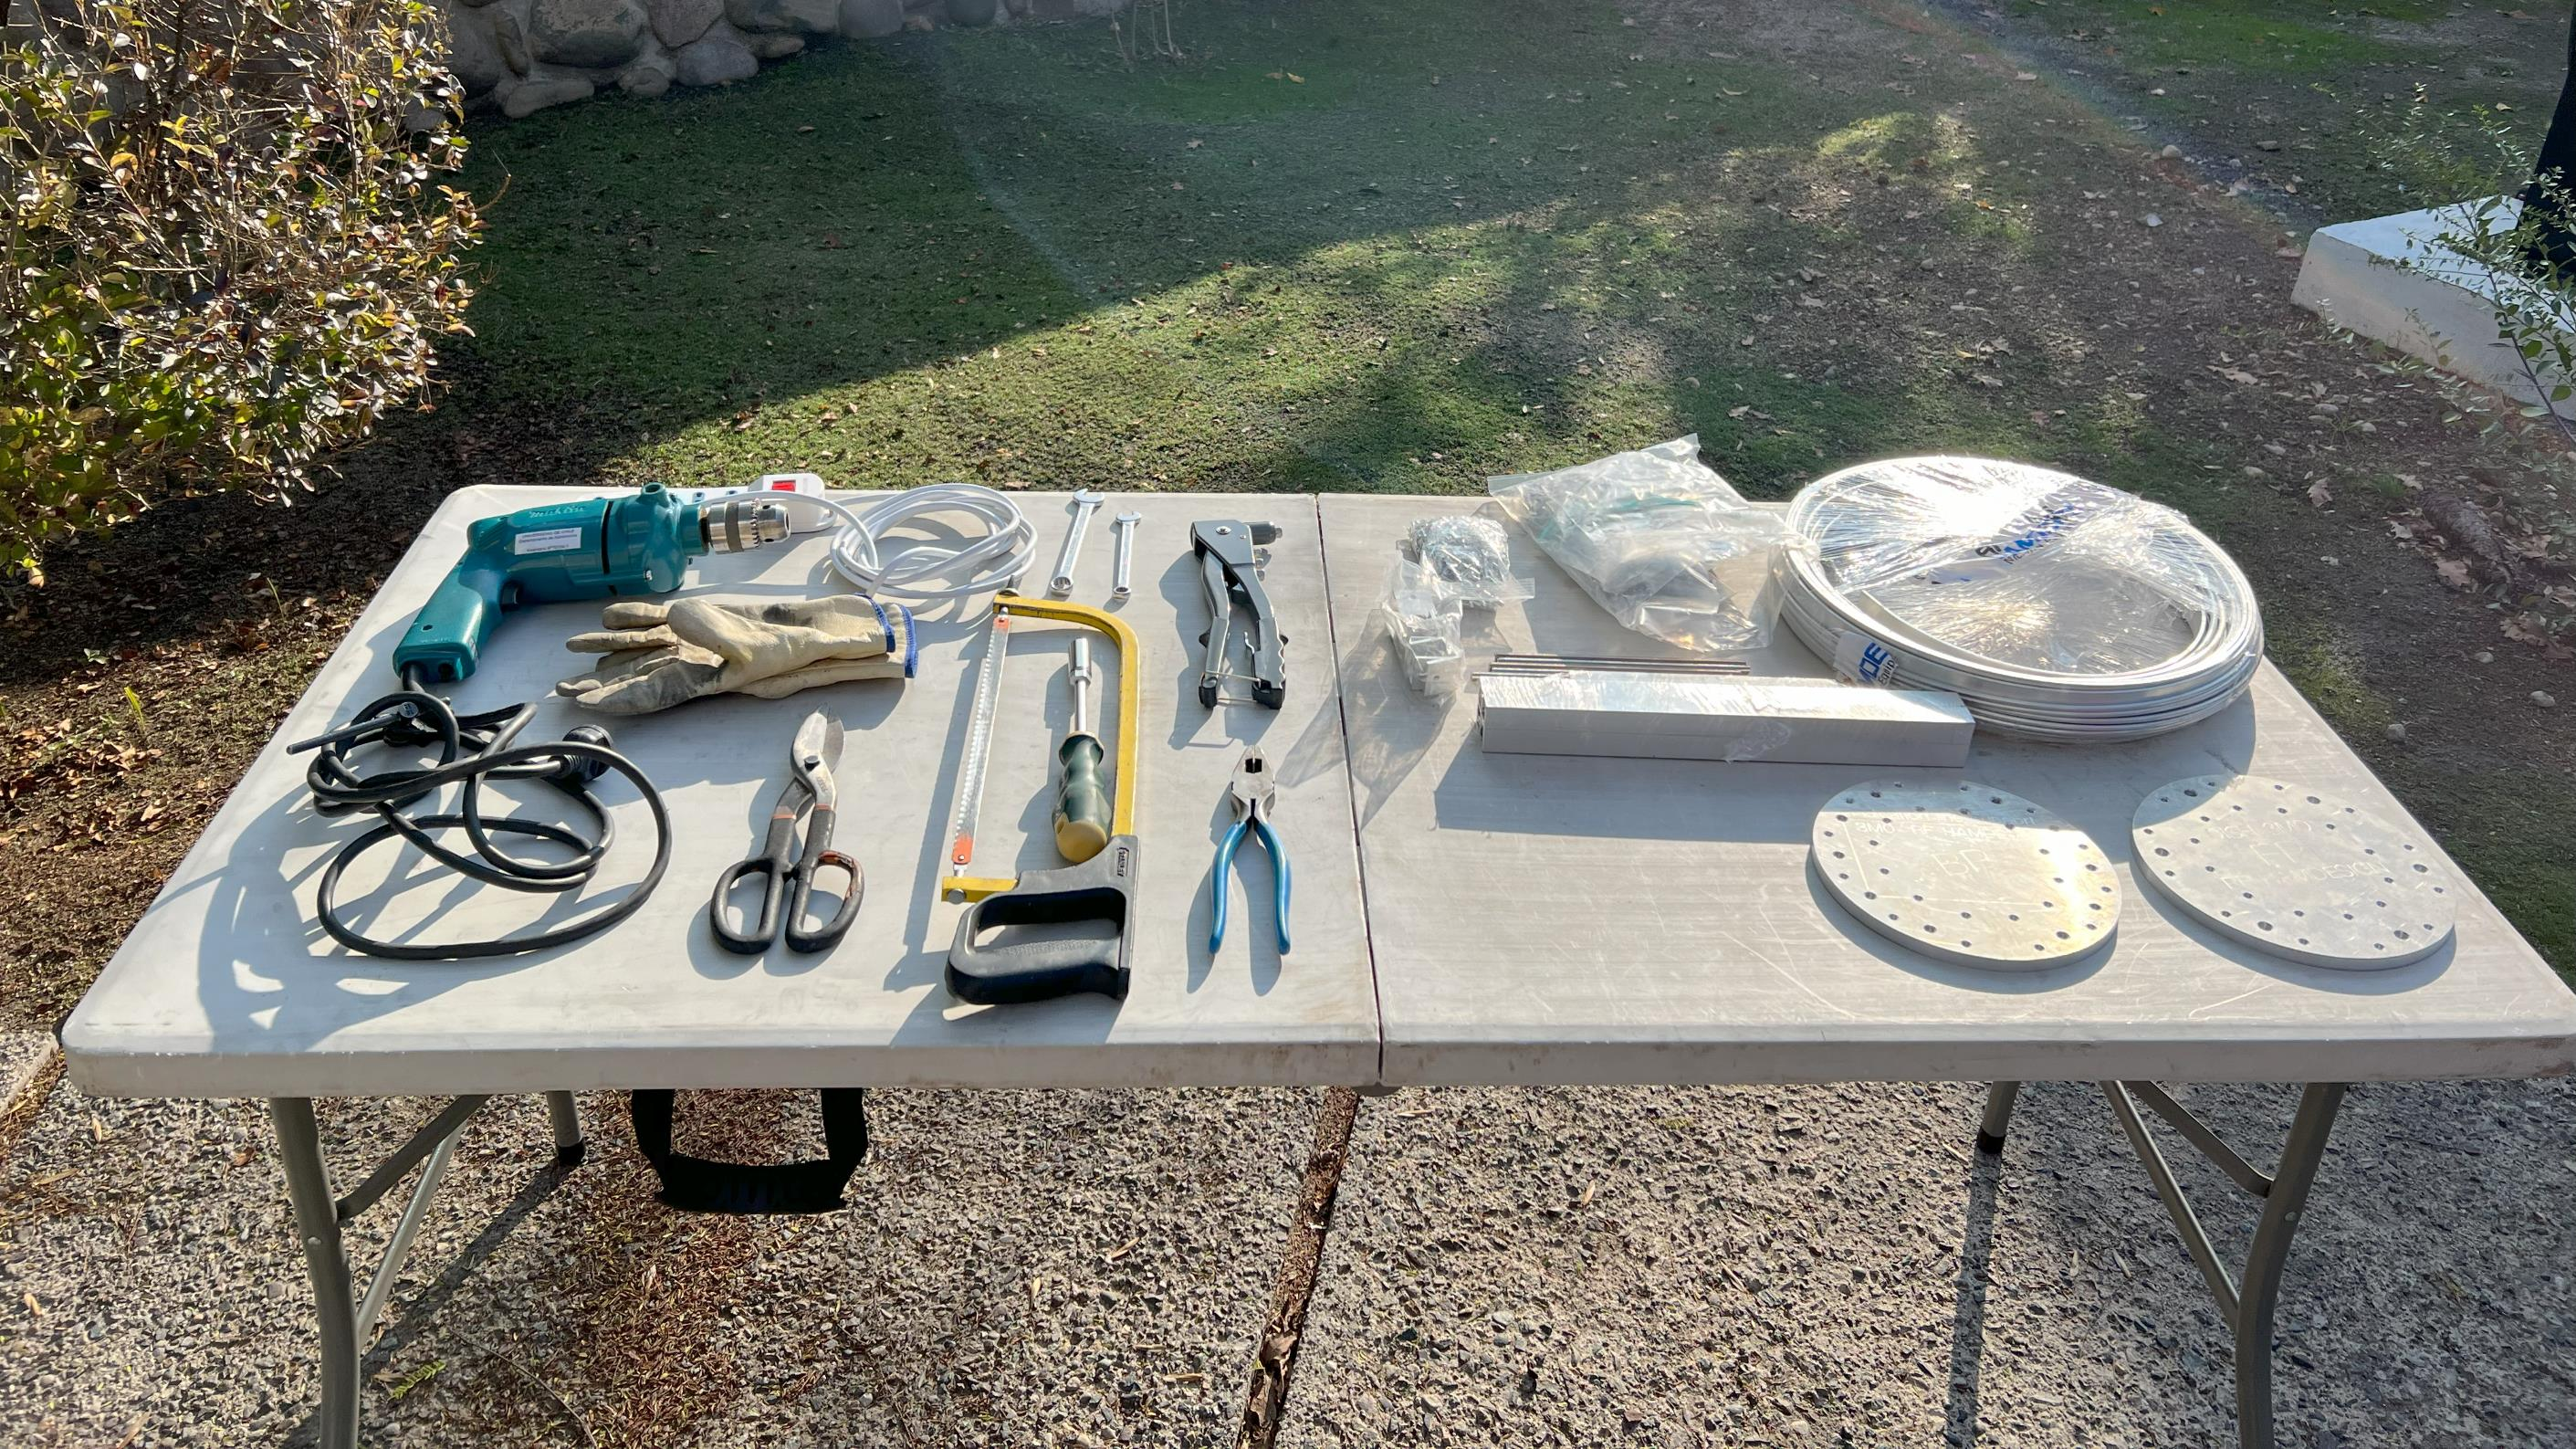
\includegraphics[width=0.8\textwidth]{img/herramientas}
    \caption{Herramientas utilizadas para el ensamblado de la superficie del reflector parabólico.}
    \label{fig:ensamblado1}
\end{figure}

En la figura \ref{fig:ensamblado1} se pueden ver las herramientas utilizadas para el ensamblado de la superficie del reflector parabólico además de las piezas que requerían de modificación adicional para la instalación correcta.\\

\subsection{Reflector Parabólico}

Las piezas del reflector se dividen en los 12 arcos, o costillas de aluminio que conforman la estructura que da forma a la superficie parabólica, con un centro de aluminio donde estas 12 piezas se unen con pernos\\

\begin{figure}
    \centering
    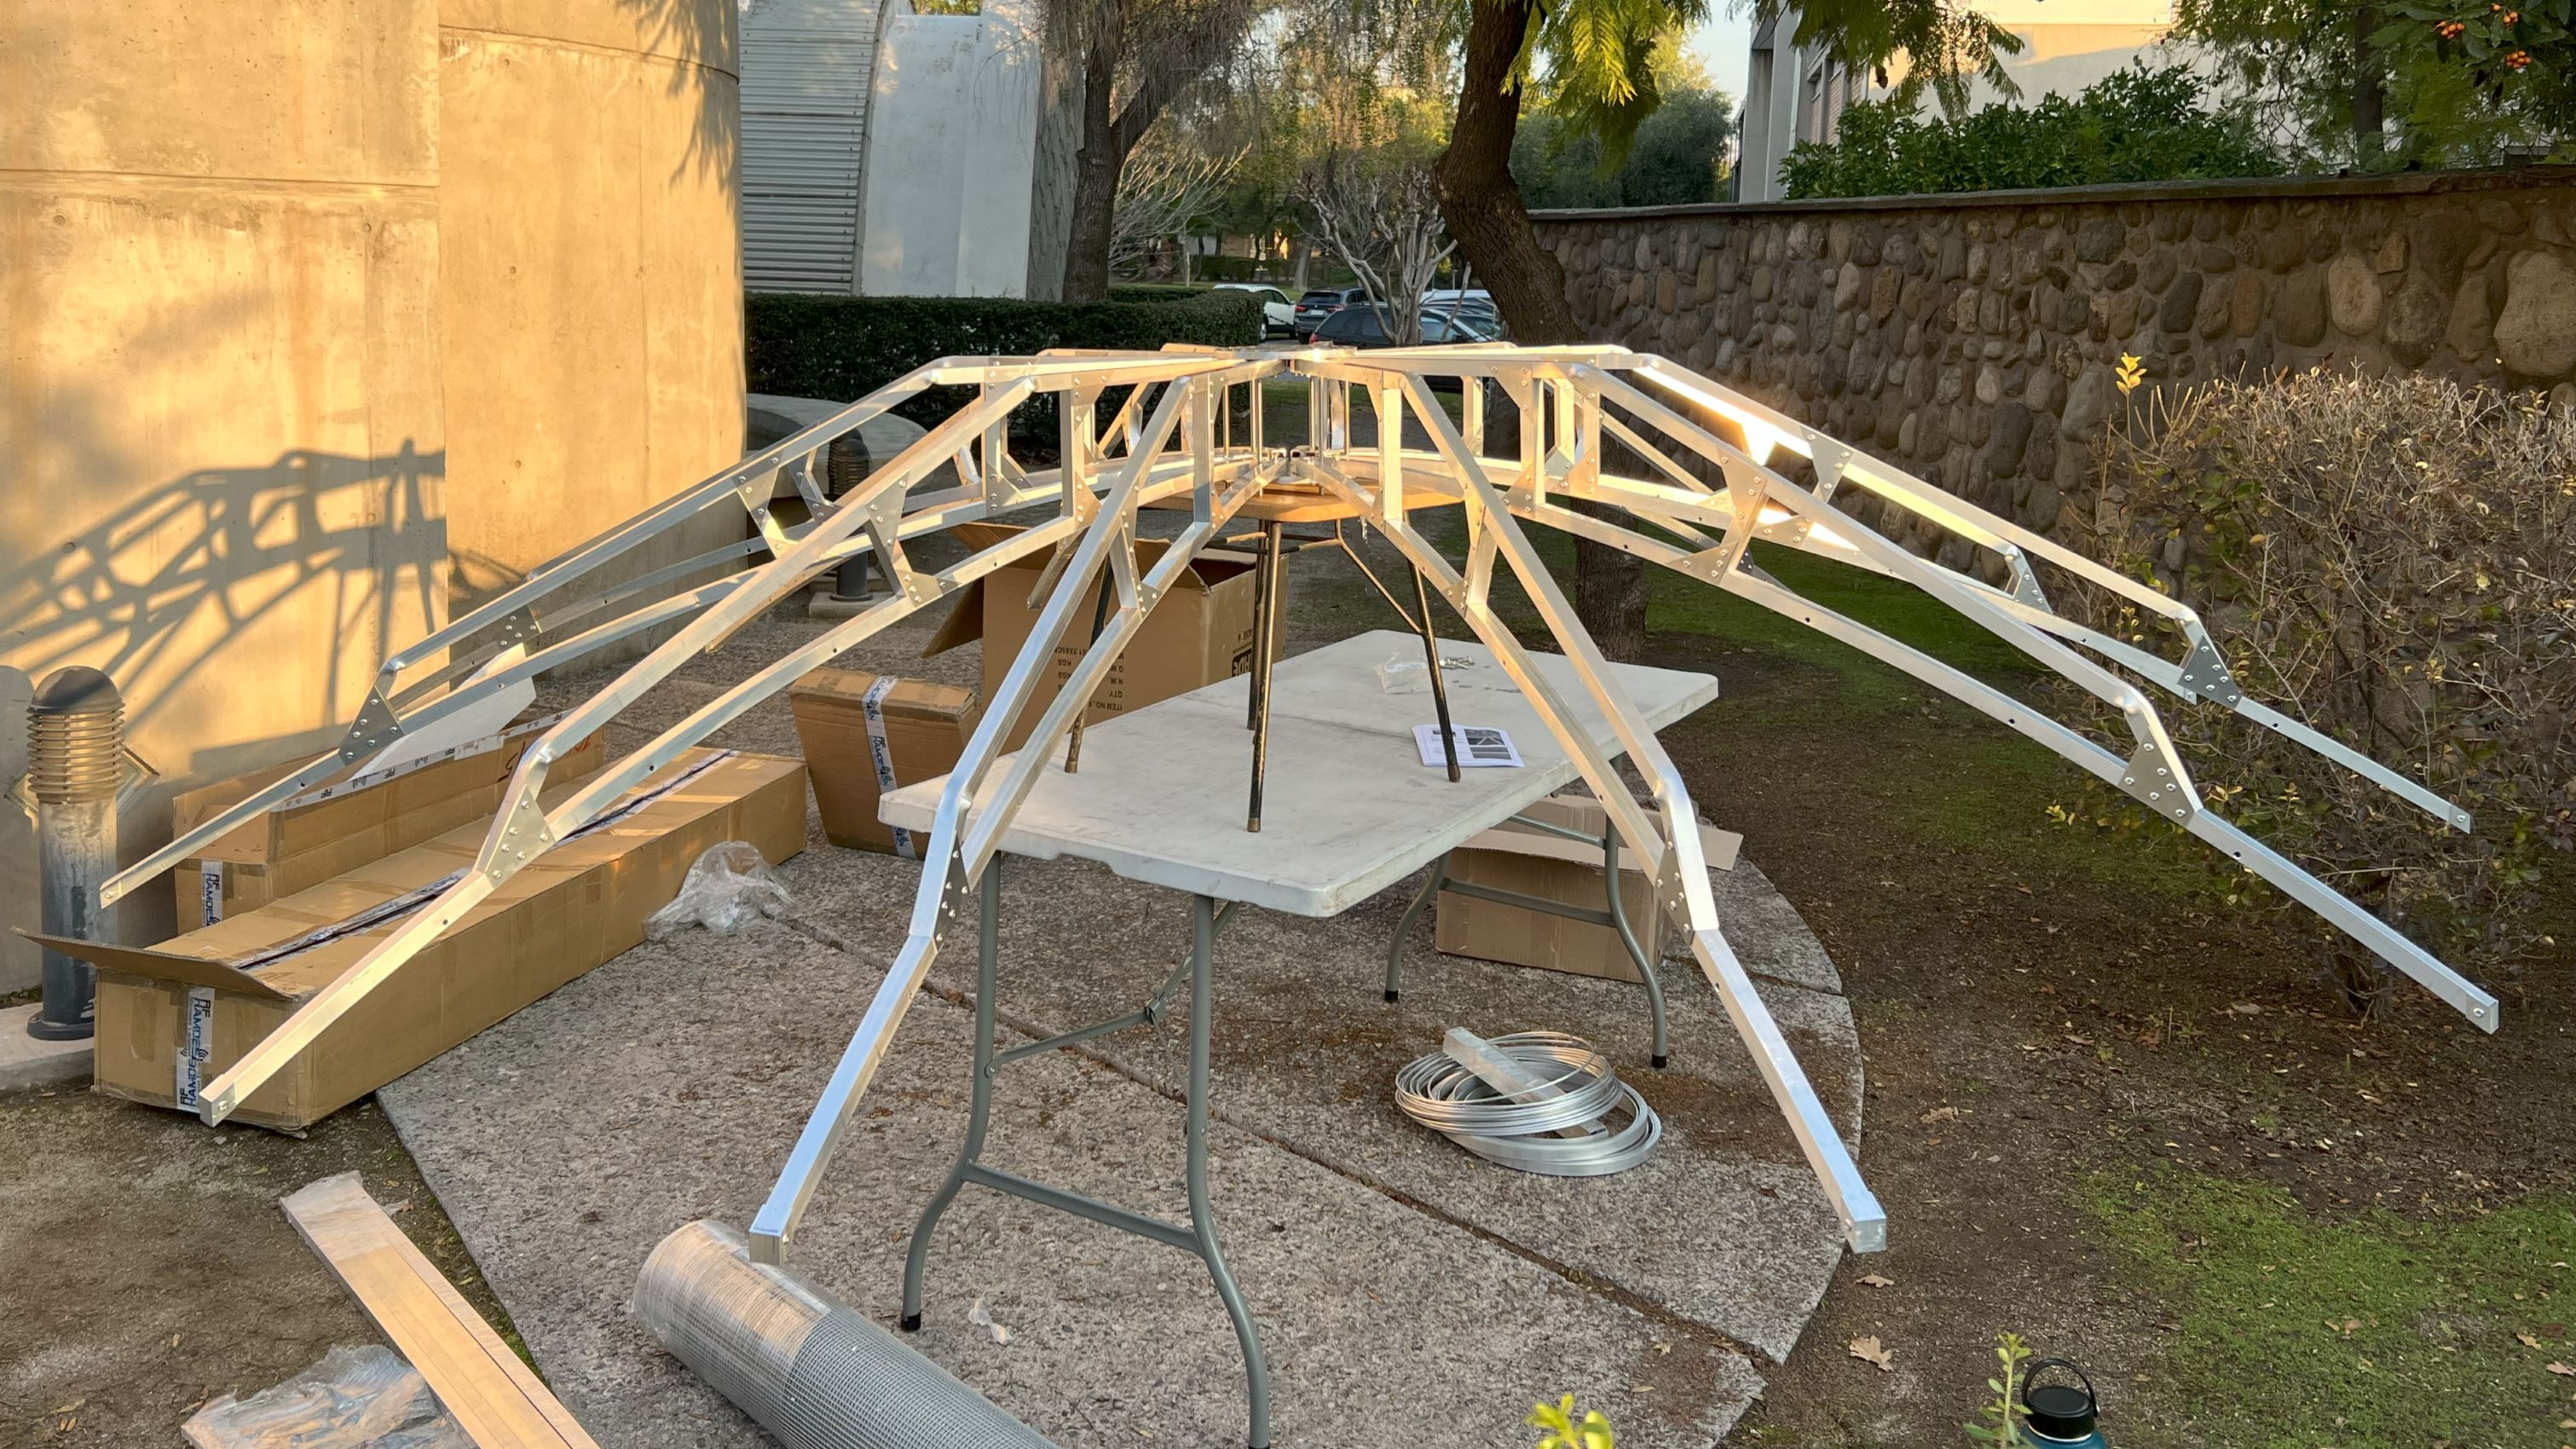
\includegraphics[width=0.8\textwidth]{img/estructura1}
    \caption{Los 12 arcos de aluminio sujetos al centro del reflector parabólico.}
    \label{fig:ensamble2}
\end{figure}

En la figura \ref{fig:ensamble2} se pueden ver los 12 arcos de aluminio sujetos a los discos de distribución, que además es el punto de anclaje para el soporte de la montura.\\

Luego se desenrollaron y enderezaron los tubos de aluminio que conforman los anillos donde se tensaron las mallas metálicas que definen la superficie del reflector. Con la misma lógica se tomó la cinta de aluminio, que es aproximadamente de 4 mm de espesor, para enderezarla y prepara las perforaciones para los primeros remaches.\\

\begin{figure}
    \centering
    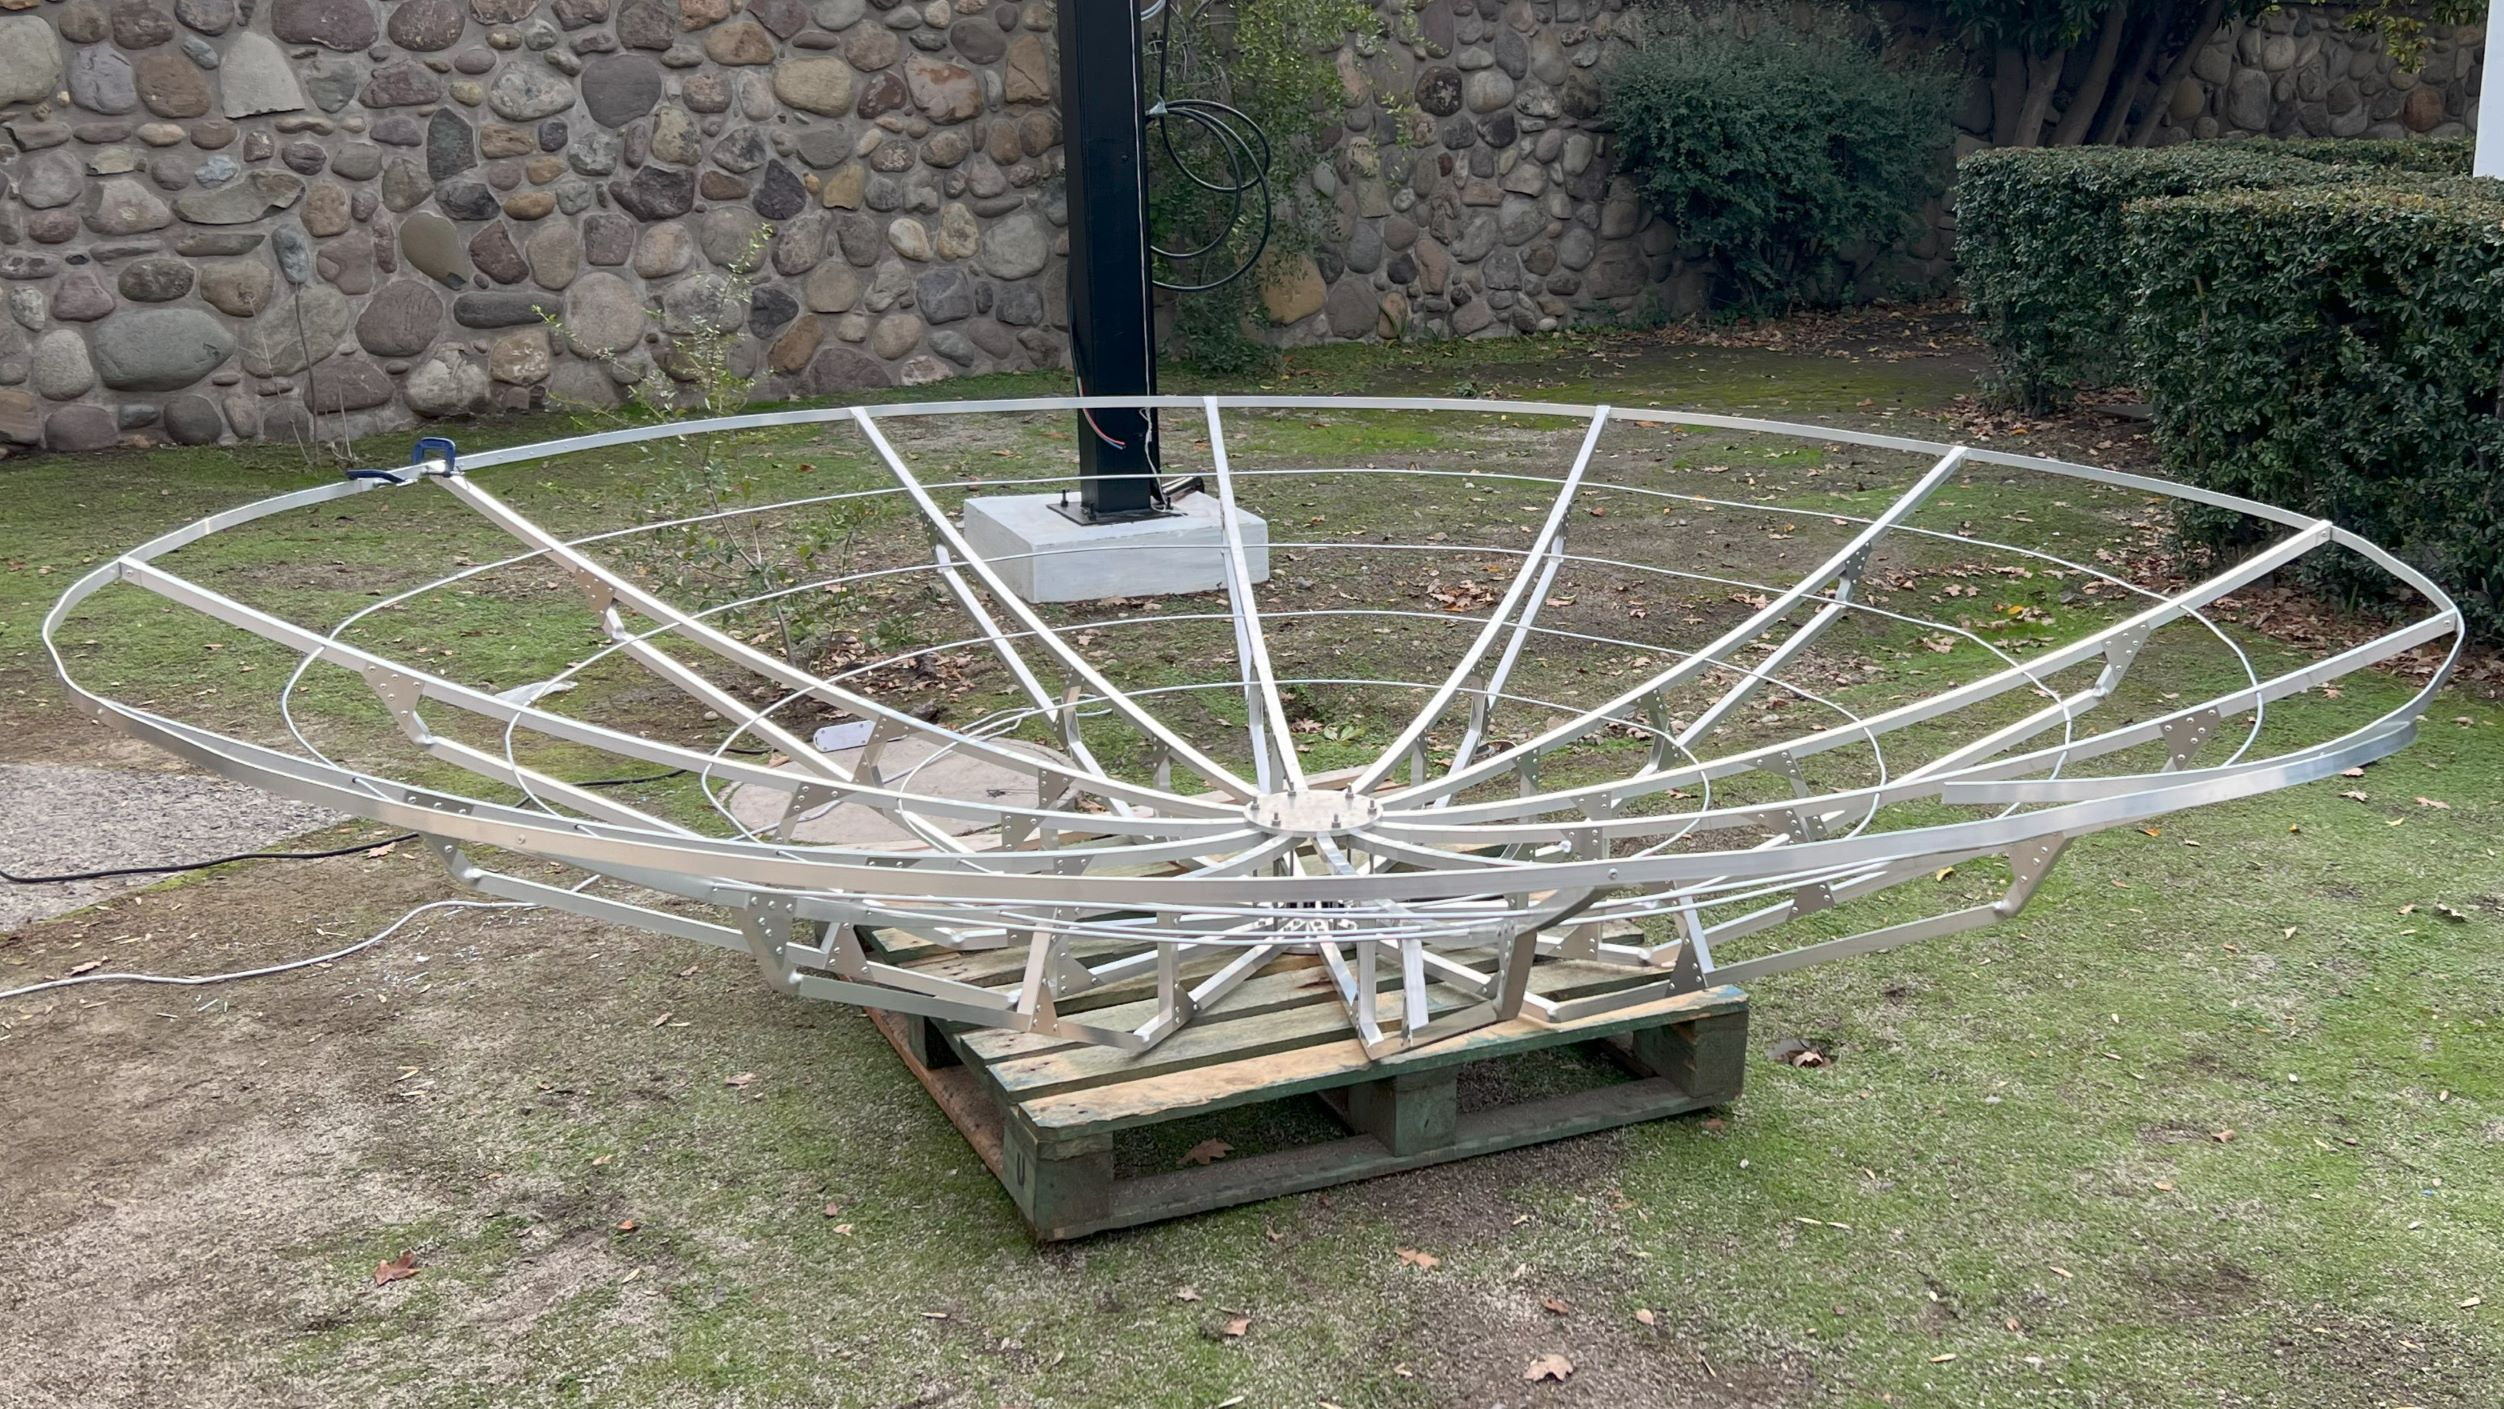
\includegraphics[width=0.8\textwidth]{img/estructura2}
    \caption{Los tubos de aluminio y la cinta de aluminio para la tensión de la malla metálica instalados radialmente en los soportes.}
    \label{fig:ensamble3}
\end{figure}

\subsection{Diagrama general del telescopio}

Por el ambito mecanico, el telescopio se compone de 4 partes principales, el relfector parabolico, la montura alt-azimutal con su rotor, el alimentador y el receptor de radiofrecuencia.\\

\begin{figure}
    \centering
    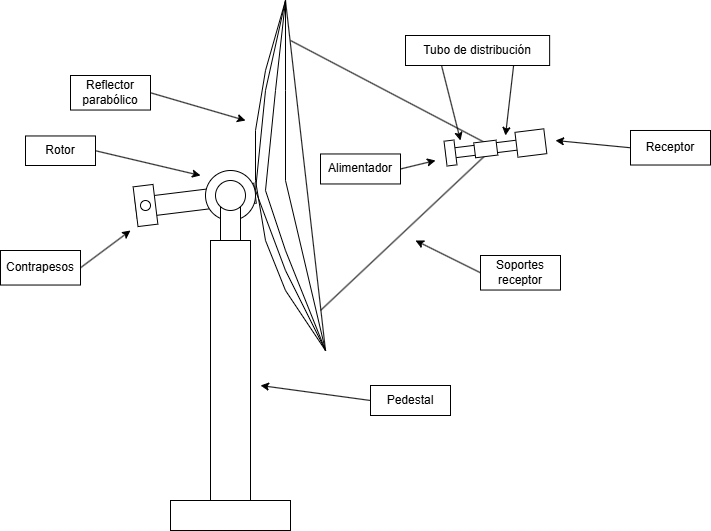
\includegraphics[width=0.8\textwidth]{img/general}
    \caption{Diagrama general del telescopio con sus componentes principales.}
    \label{fig:ensambleGen}
\end{figure}

En la figura \ref{fig:ensambleGen} se puede ver como se enamblan cada una de las piesas del telescopio de forma conceptual, sin embargo, en la práctica se requiere de soportes adicionales para poder asegurar cada una de las piezas. En la siguiente sección se detallarán los soportes adicionales diseñados e impresos en 3D para el telescopio.\\

\subsection{Diseño de soportes adicionales}


Para poder instalar todos los componentes del telescopio, se debió fabricar soportes personalizados y adicionales para así poder utilizar receptores y elementos que no fueran parte del kit original del fabricante. Con el objetivo de reducir los tiempos de fabricación y prototipado al usar componentes de aluminio o acero se decidió utilizar impresión 3D con filamento plástico PLA\footnote{PLA del inglés Ácido Poliláctico, es un termo plástico sostenible utilizado en la impresión 3D} de alta resistencia mecánica.\\

Se diseñaron 6 piezas en total con el software de diseño asistido por computadora o \textit{CAD} \textit{Fusion 360} de la compañía \textit{Autodesk}. Todos los componentes fueron impresos en PLA de alta resistencia o \textit{Hyper-PLA} de la compañía \textit{Creality}, otorgando una mayor resistencia a la flexión de 50\% que el PLA convencional y una elongación de 6.304\% en comparación con la del PLA convencional de 3\%. La configuración de la impresión fue una altura de capa de 0.2 mm, dada por la boquilla utilizada, 4 capas de muralla y un \textit{Infill} o relleno de 60 \%.\\

Una ventaja importante en la elección de la impresión 3D en filamentos plásticos, es su baja incidencia en la deformación o interferencia del comportamiento de radiofrecuencia, al ser un material no conductor introducido en el campo cercano de los componentes.\\

Se puende consultar los dibujos mecanicos con medidas y carateristicas en el anexo. \ref{anexo:soportes_patas}.\\

\begin{figure}
    \centering
    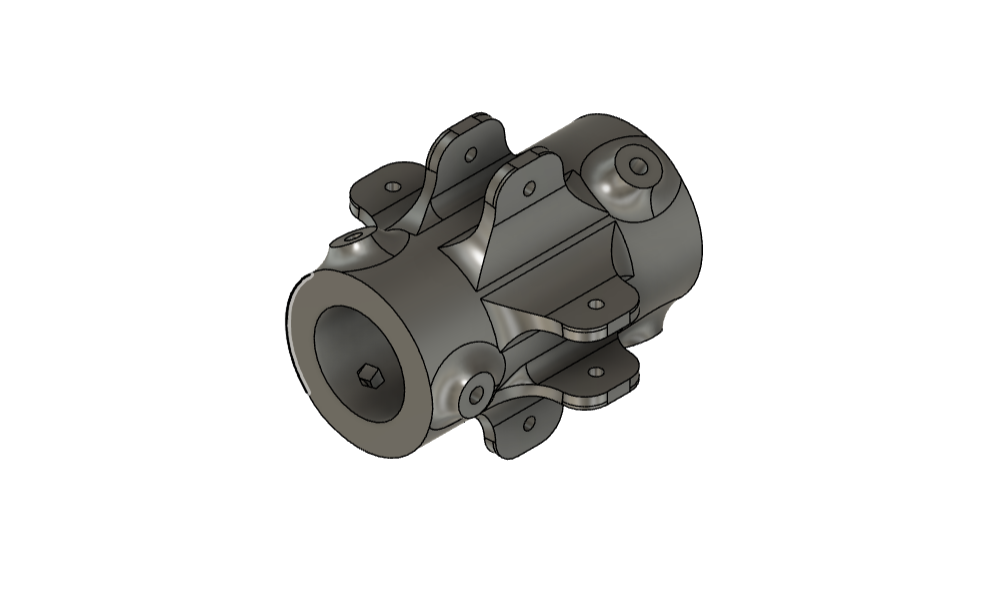
\includegraphics[width=0.8\textwidth]{img/soporte3D5}
    \caption{Unión de los soportes de aluminio para el alimentador.}
    \label{fig:ensamble4}
\end{figure}

El diseño 3D de la figura \ref{fig:ensamble4} es un soporte que contiene una cavidad centrar cilíndrica que cumple la función de sostener tanto el alimentador como el receptor por medio de un tubo plástico de PVC\footnote{PVC, cloruro de polivinilo, polimero plástico} que asegura que todo se mantenga alineado con el centro de la parábola, además de permitir un movimiento en el eje de la cavidad cilíndrica para ajustar el foco del alimentador.\\

Tiene 4 ranuras perforadas para asegurar los soportes con pernos M4 de medida y también 6 perforaciones con cavidades para tuercas M5. Con estas tuercas y con los respectivos tornillos se asegura la posición del tubo de PVC para fijar el foco una vez encontrado.\\

Las siguientes piezas comparten la misma filosofía de diseño, para poder ser compatibles entre ellas y con el resto de los componentes del telescopio. Además, permiten el rediseño de nuevas piezas para otros alimentadores, cambios de largo en el tubo distribuidor de PVC y en la elección de otro material de impresión 3D si se quisiese.\\

\begin{figure}
    \centering
    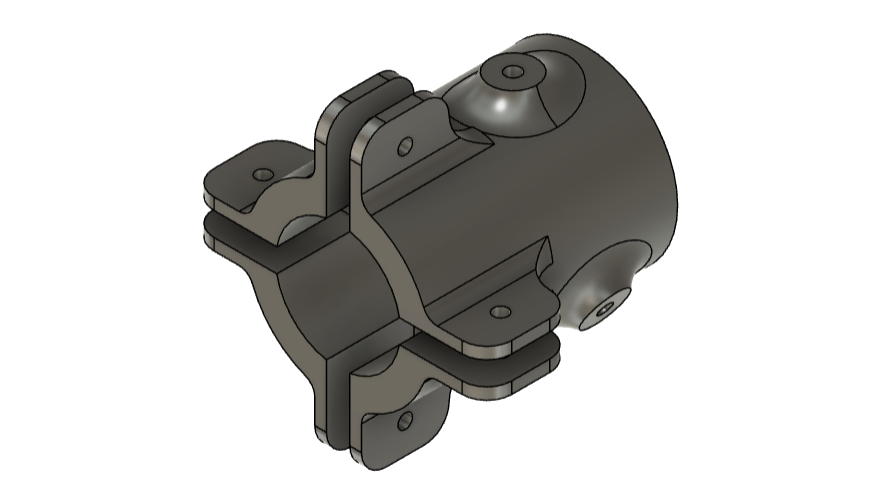
\includegraphics[width=0.8\textwidth]{img/soporte3D1v1}
    \caption{Interfaz de soporte para el tubo de distribución y otros elementos}
    \label{fig:ensamble5}
\end{figure}

La figura \ref{fig:ensamble5} es un soporte multipropósito que permite acoplar otros soportes de menor complejidad para ser instalados en la zona del alimentador y receptor. Así permite cambios en la instrumentación que se requiera en el futuro sin tener que rediseñar toda la estructura de sujeción.\\

\begin{figure}
    \centering
    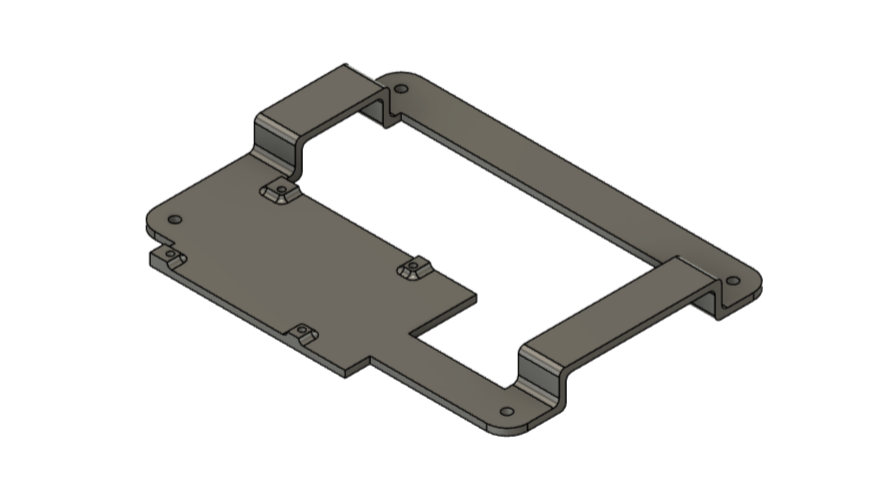
\includegraphics[width=0.8\textwidth]{img/soporte3D7}
    \caption{Soporte interno para electrónica de recepción}
    \label{fig:ensamble6}
\end{figure}

El receptor de radiofrecuencia se encuentra dentro de una caja eléctrica a prueba de agua, pero se requiere un soporte interno para asegurar que la placa de adquisición de datos y el digitalizador se mantengan en su lugar mientras el telescopio se mueve en distintas elevaciones. La figura \ref{fig:ensamble6} es un soporte que se instala en la caja eléctrica y permite montar diferentes tipos de receptores y amplificadores.\\

\begin{figure}
    \centering
    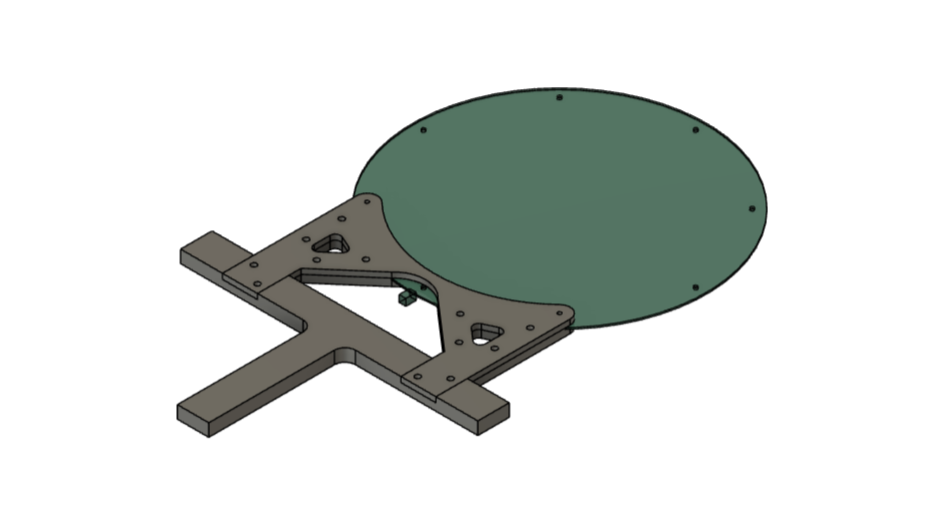
\includegraphics[width=0.8\textwidth]{img/soporte3D4}
    \caption{Soporte para la fuente de calibración de la copa de agua \quotes{estrella artificial}}
    \label{fig:ensamble7}
\end{figure}

La figura \ref{fig:ensamble7} es un soporte que fue diseñado para instalar la fuente de calibración de la copa de agua o \quotes{estrella artificial} en parte superior de la copa de agua del cerro Calán. Se divide en 2 piezas que se unen por medio de pernos M4 de plástico para sujetar la antena circular por presión y con tornillos pasantes. Además, para poder asegurar este soporte con facilidad y rapidez, se diseñó la forma de cruz para que por medio de amarras plásticas se pueda asegurar a la baranda de la copa de agua.\\

\begin{figure}
    \centering
    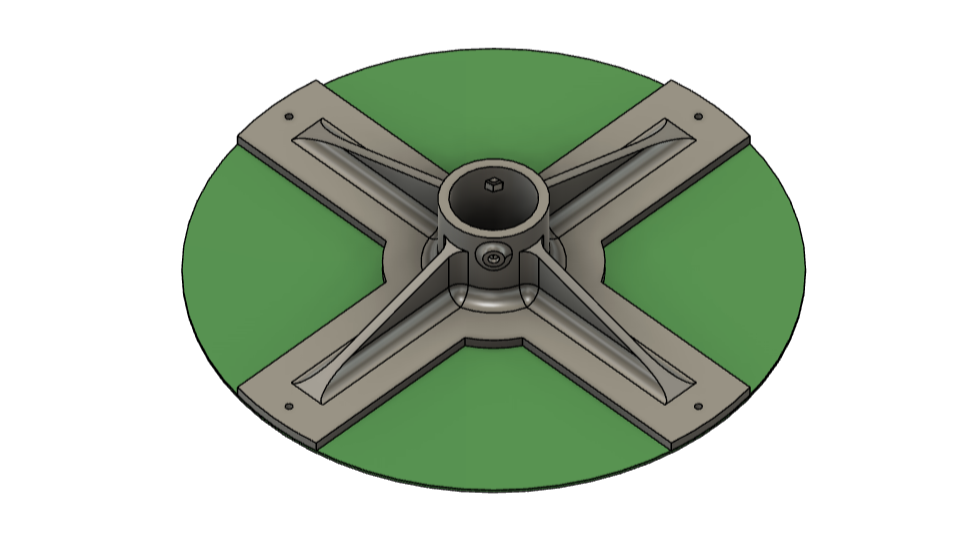
\includegraphics[width=0.8\textwidth]{img/soporte3D2}
    \caption{Soporte para antena circular de alto ancho de banda para configuración de alimentador}
    \label{fig:ensamble8}
\end{figure}

Para las mediciones de baja frecuencia (menores a 600 MHz) se debe utilizar la misma antena circular de la figura \ref{fig:ensamble7} pero con un soporte diferente. La figura \ref{fig:ensamble8} es un soporte que permite colocar la antena como alimentador del telescopio por medio del tubo de PVC y asegurarla con pernos M4 al este y pernos plásticos M3 para la antena y el soporte.\\

\begin{figure}
    \centering
    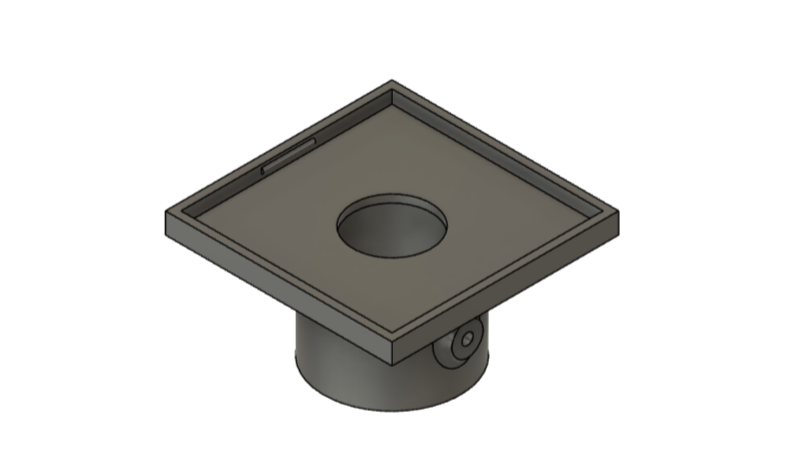
\includegraphics[width=0.8\textwidth]{img/soporte3D6}
    \caption{Soporte para el dipolo exótico como alimentador de 1420 MHz}
    \label{fig:ensamble9}
\end{figure}

Al igual que en la figura \ref{fig:ensamble8}, la figura \ref{fig:ensamble9} es un soporte que permite colocar el dipolo exótico como alimentador del telescopio por medio del tubo de PVC. Diferenciándose del soporte anterior, este diseño permite asegurar la placa de la antena con la deformación forzada del material impreso, evitando el uso de pernos y tuercas.\\

\subsection{Montura Alt-Azimutal}

El rotor utilizado para la montura alt-azimutal es el modelo \textit{BIG-RAS/HR} de la compañía \textit{RFHamdesign} está diseñado para soportar una carga de hasta 319 kg, con una velocidad de movimiento de hasta 2.5 grados por segundo y una resolución de 0.1 grados para sus codificadores de posición.\\

\begin{figure}
    \centering
    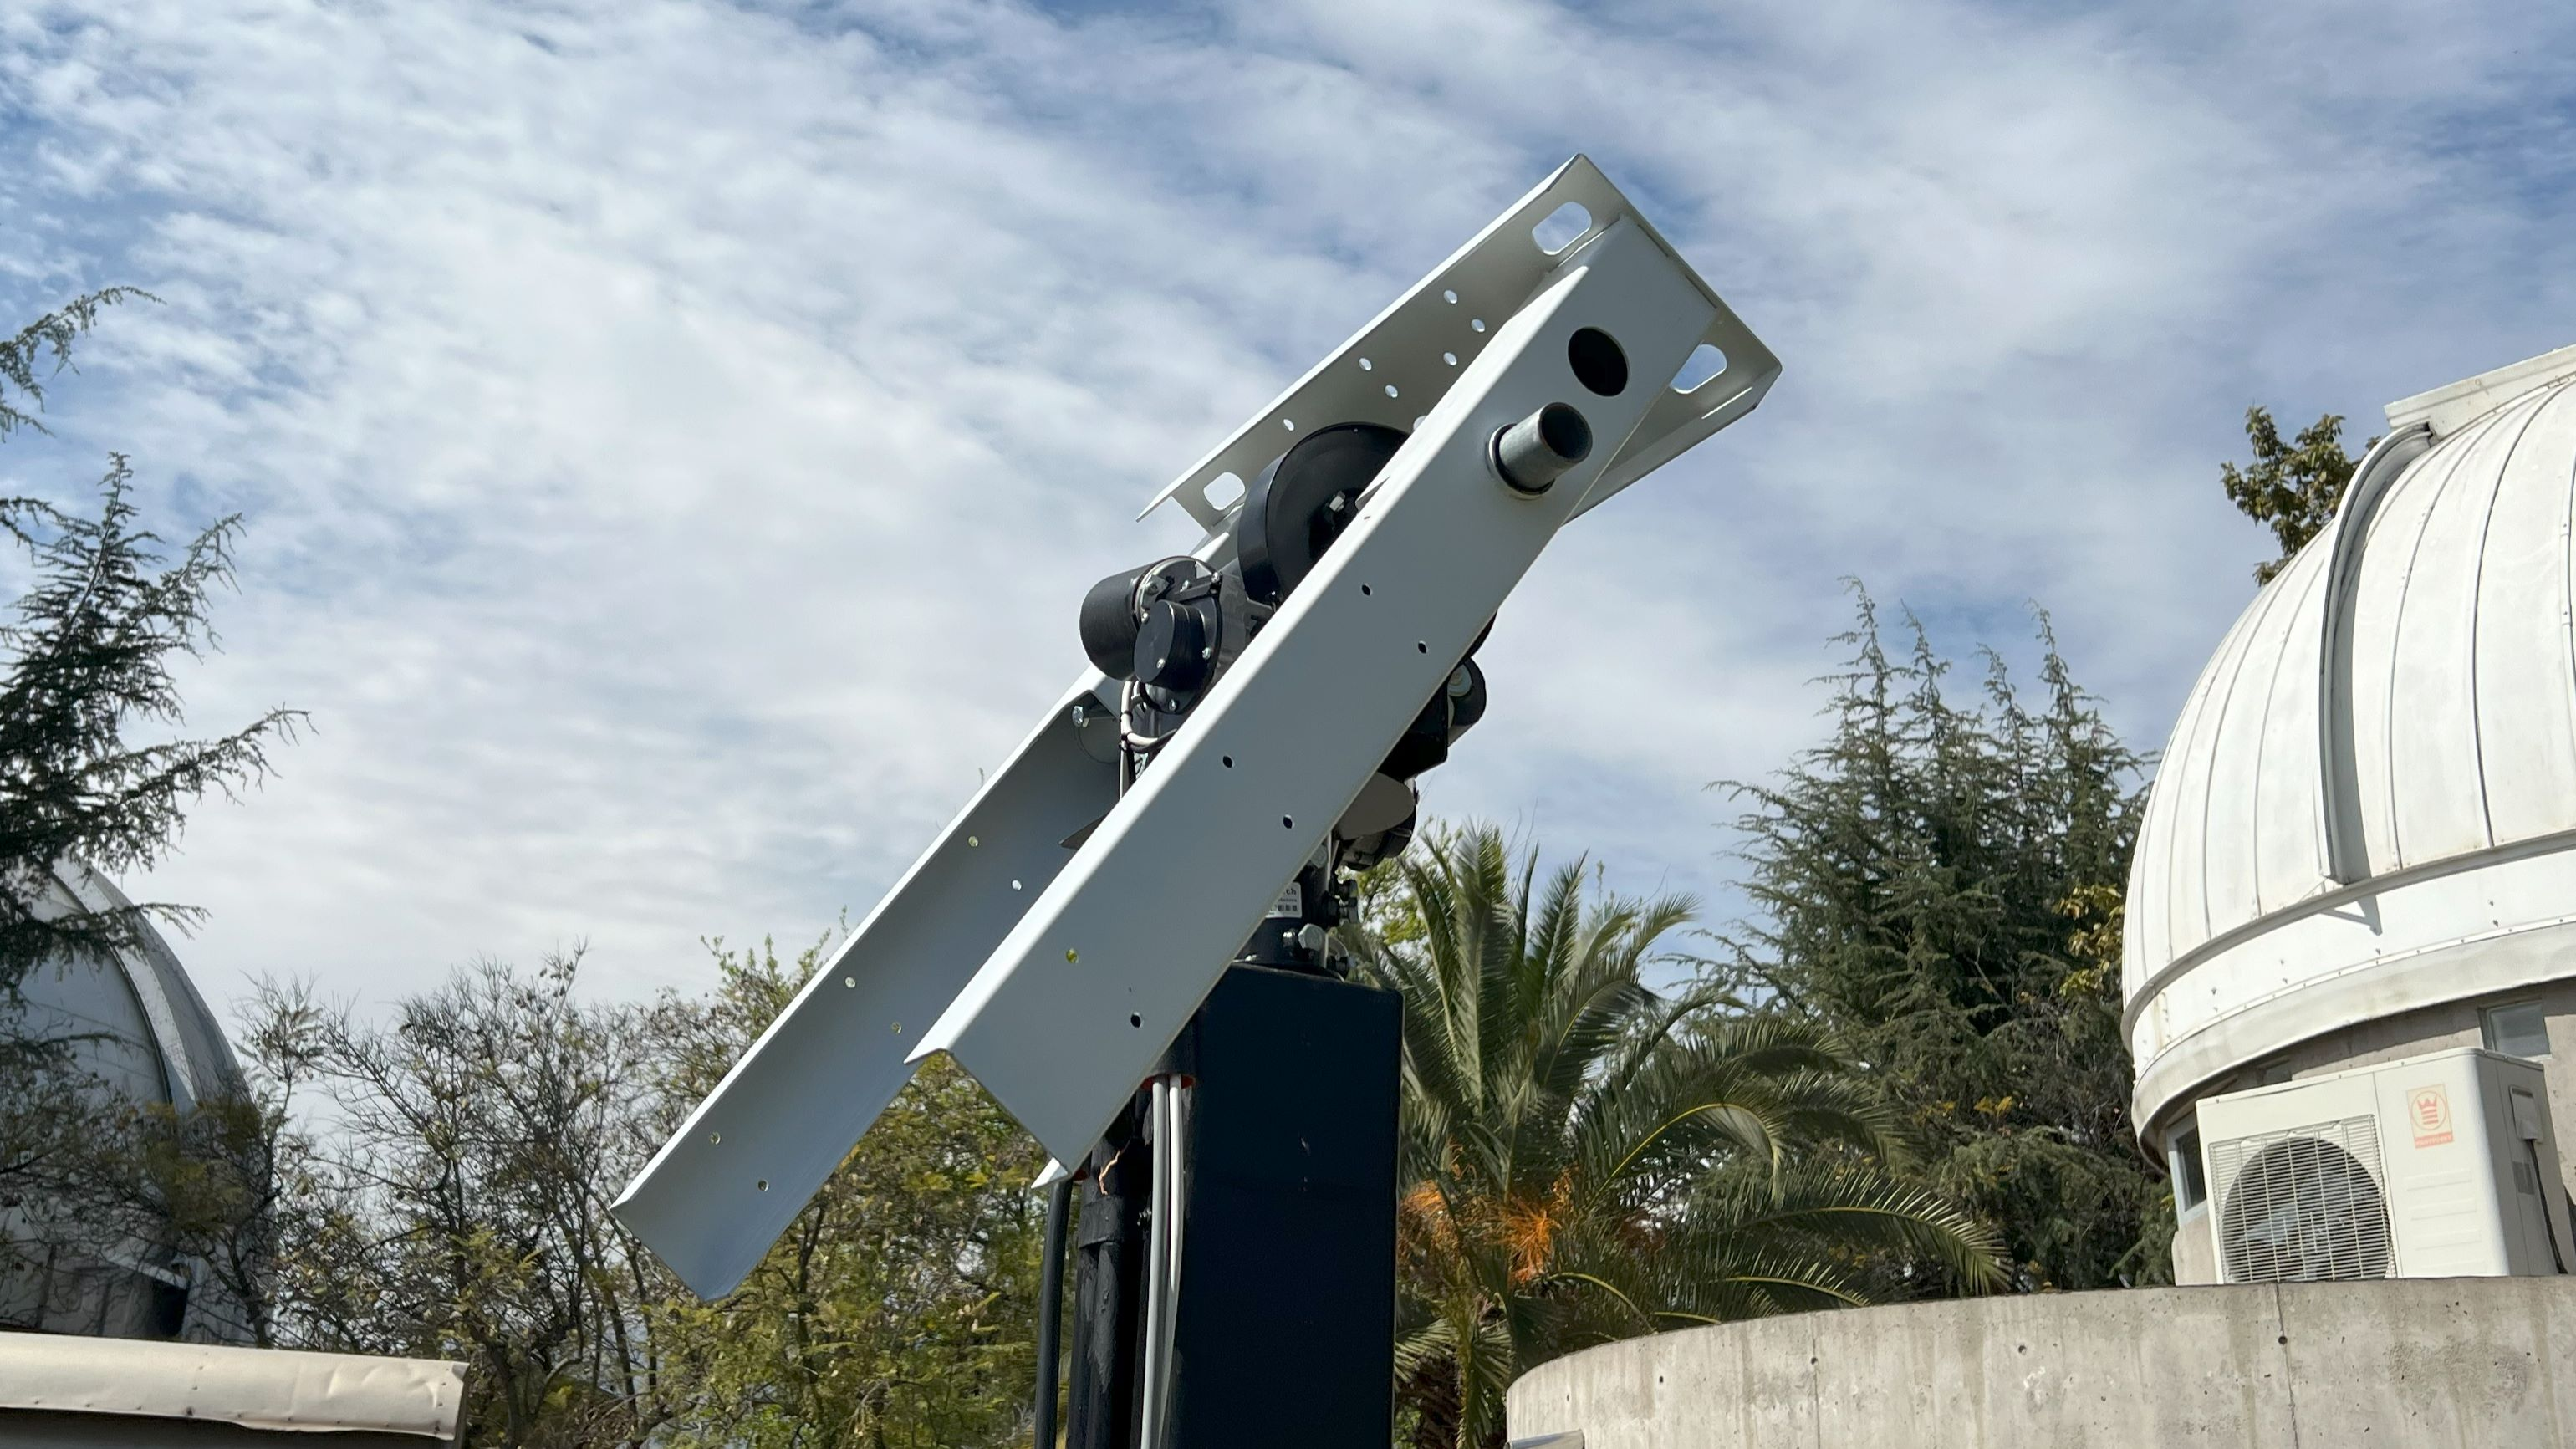
\includegraphics[width=0.8\textwidth]{img/soporte_montura}
    \caption{Rotor \textit{BIG-RAS/HR} de la compañía \textit{RFHamdesign} instalada en el pedestal con la montura de acero.}
    \label{fig:ensamble10}
\end{figure}

En la figura \ref{fig:ensamble10} se puede ver el rotor instalado en el pedestal de acero con la montura que hace la interfaz entre los motores y el reflector. La montura tiene unos brazos traseros perforados para instalar los contrapesos de equilibrio y compensar el torque que ejerce la masa del reflector. La pieza que une la montura con el rotor es una tubería de acero galvanizado de 46.5 mm de diámetro, cortada a la medida de la montura. Todos los pernos de sujeción son M10 de cabeza hexagonal.\\

\begin{figure}
    \centering
    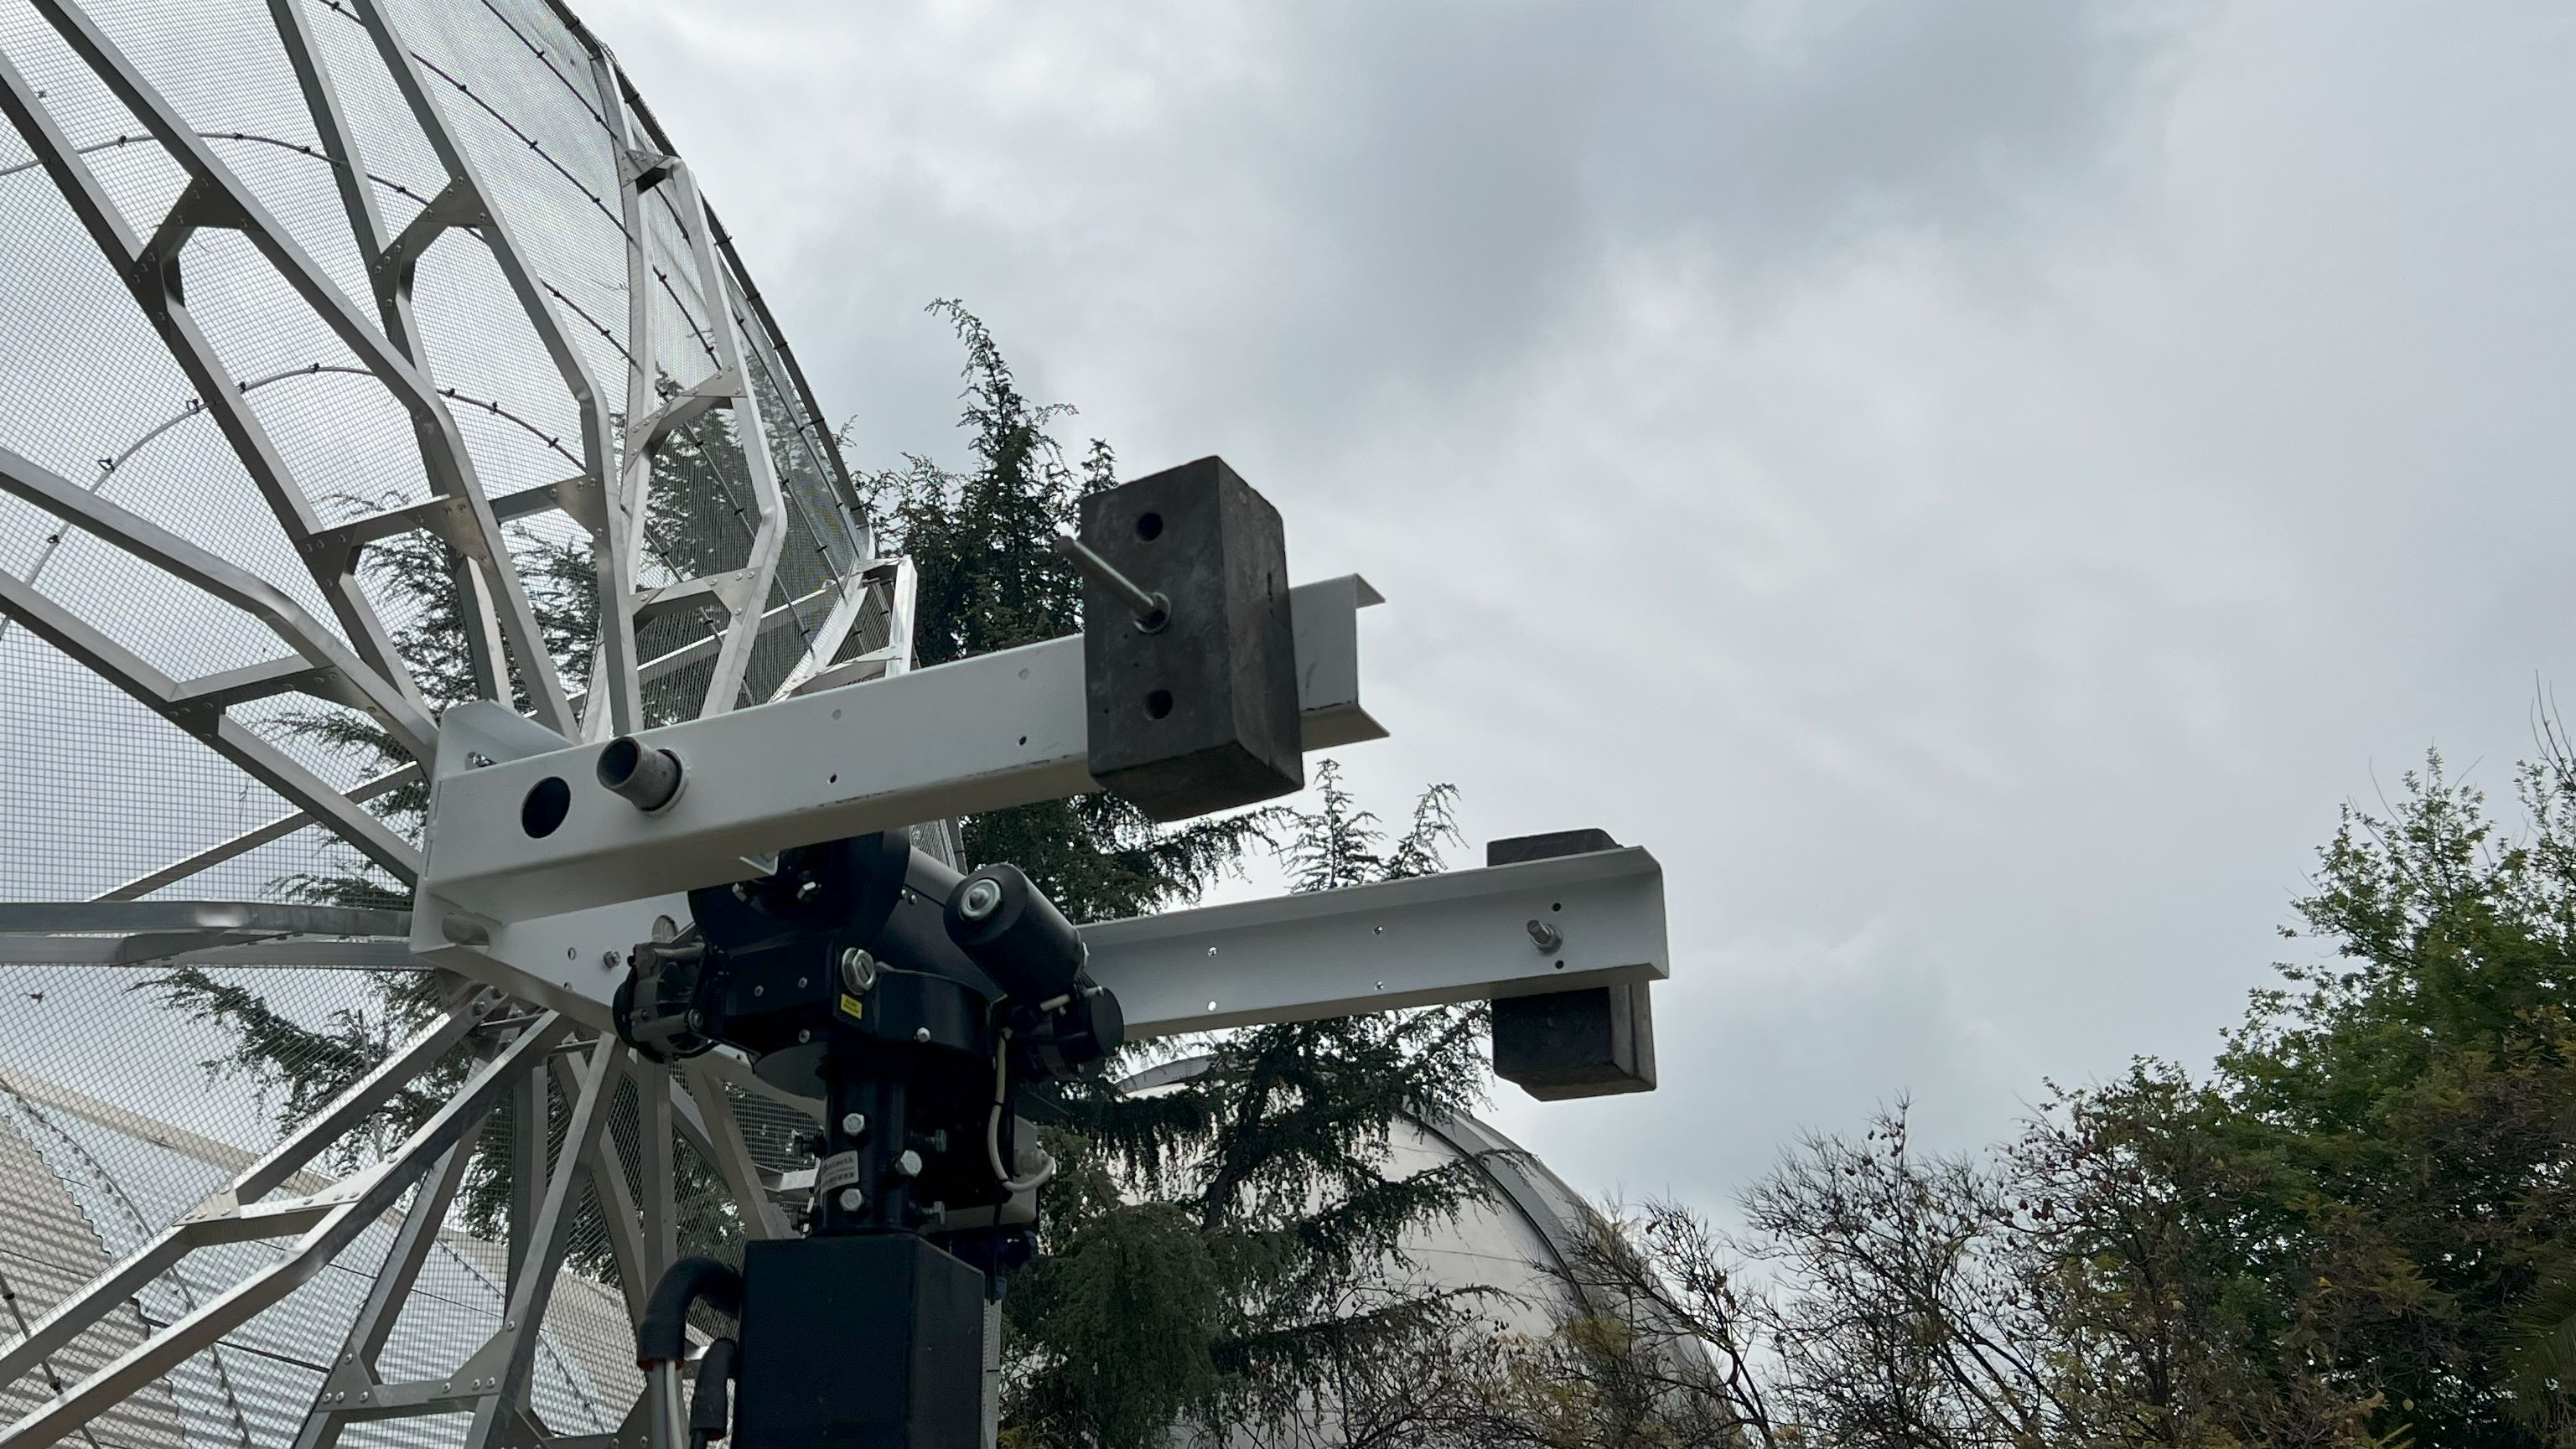
\includegraphics[width=0.8\textwidth]{img/contrapesos}
    \caption{Montura de acero con los contrapesos de equilibrio instalados.}
    \label{fig:ensamble11}
\end{figure}

En la figura \ref{fig:ensamble11} se pueden ver los contrapesos de equilibrio instalados en la montura de acero. Los contrapesos son ladrillos de una mezcla de plomo y cemento de 10 kg cada uno. Se instalaron 4 ladrillos en total a una distancia de 78 cm de del eje con la tubería, lugar donde sin ejercer ninguna fuerza sobre la antena o la montura se equilibra con los pernos de sujeción completamente desajustados.\\

La montura es capaz de moverse en 400 grados en azimuth y 180 grados en elevación, con un rango de movimiento de -40 a 360 en los motores horizontales y de 0 a 180 para los motores verticales. Los cuales para mantener rangos de seguridad la montura se mueve entre 0 a 180 grados en azimuth y elevación, así se minimiza el riesgo de enrollado de los cables al girar. En la sección de software se explicará el funcionamiento del algoritmo de movimiento.\\

\subsection{Rack de control}

El rack de control se encuentra en el edificio más cercano al telescopio, el edificio del meridiano, donde también se encuentra el telescopio ARTE. El rack consiste en un gabinete de 12 unidades de rack o \textit{U} completamente de acero tanto su cuerpo como la puerta frontal. Con el objetivo de minimizar el RFI que pueda ser introducido por los componentes electrónicos, se utilizó un gabinete completamente cerrado y con una puerta frontal de acero conectado a la tierra local.\\


\begin{figure}
    \centering
    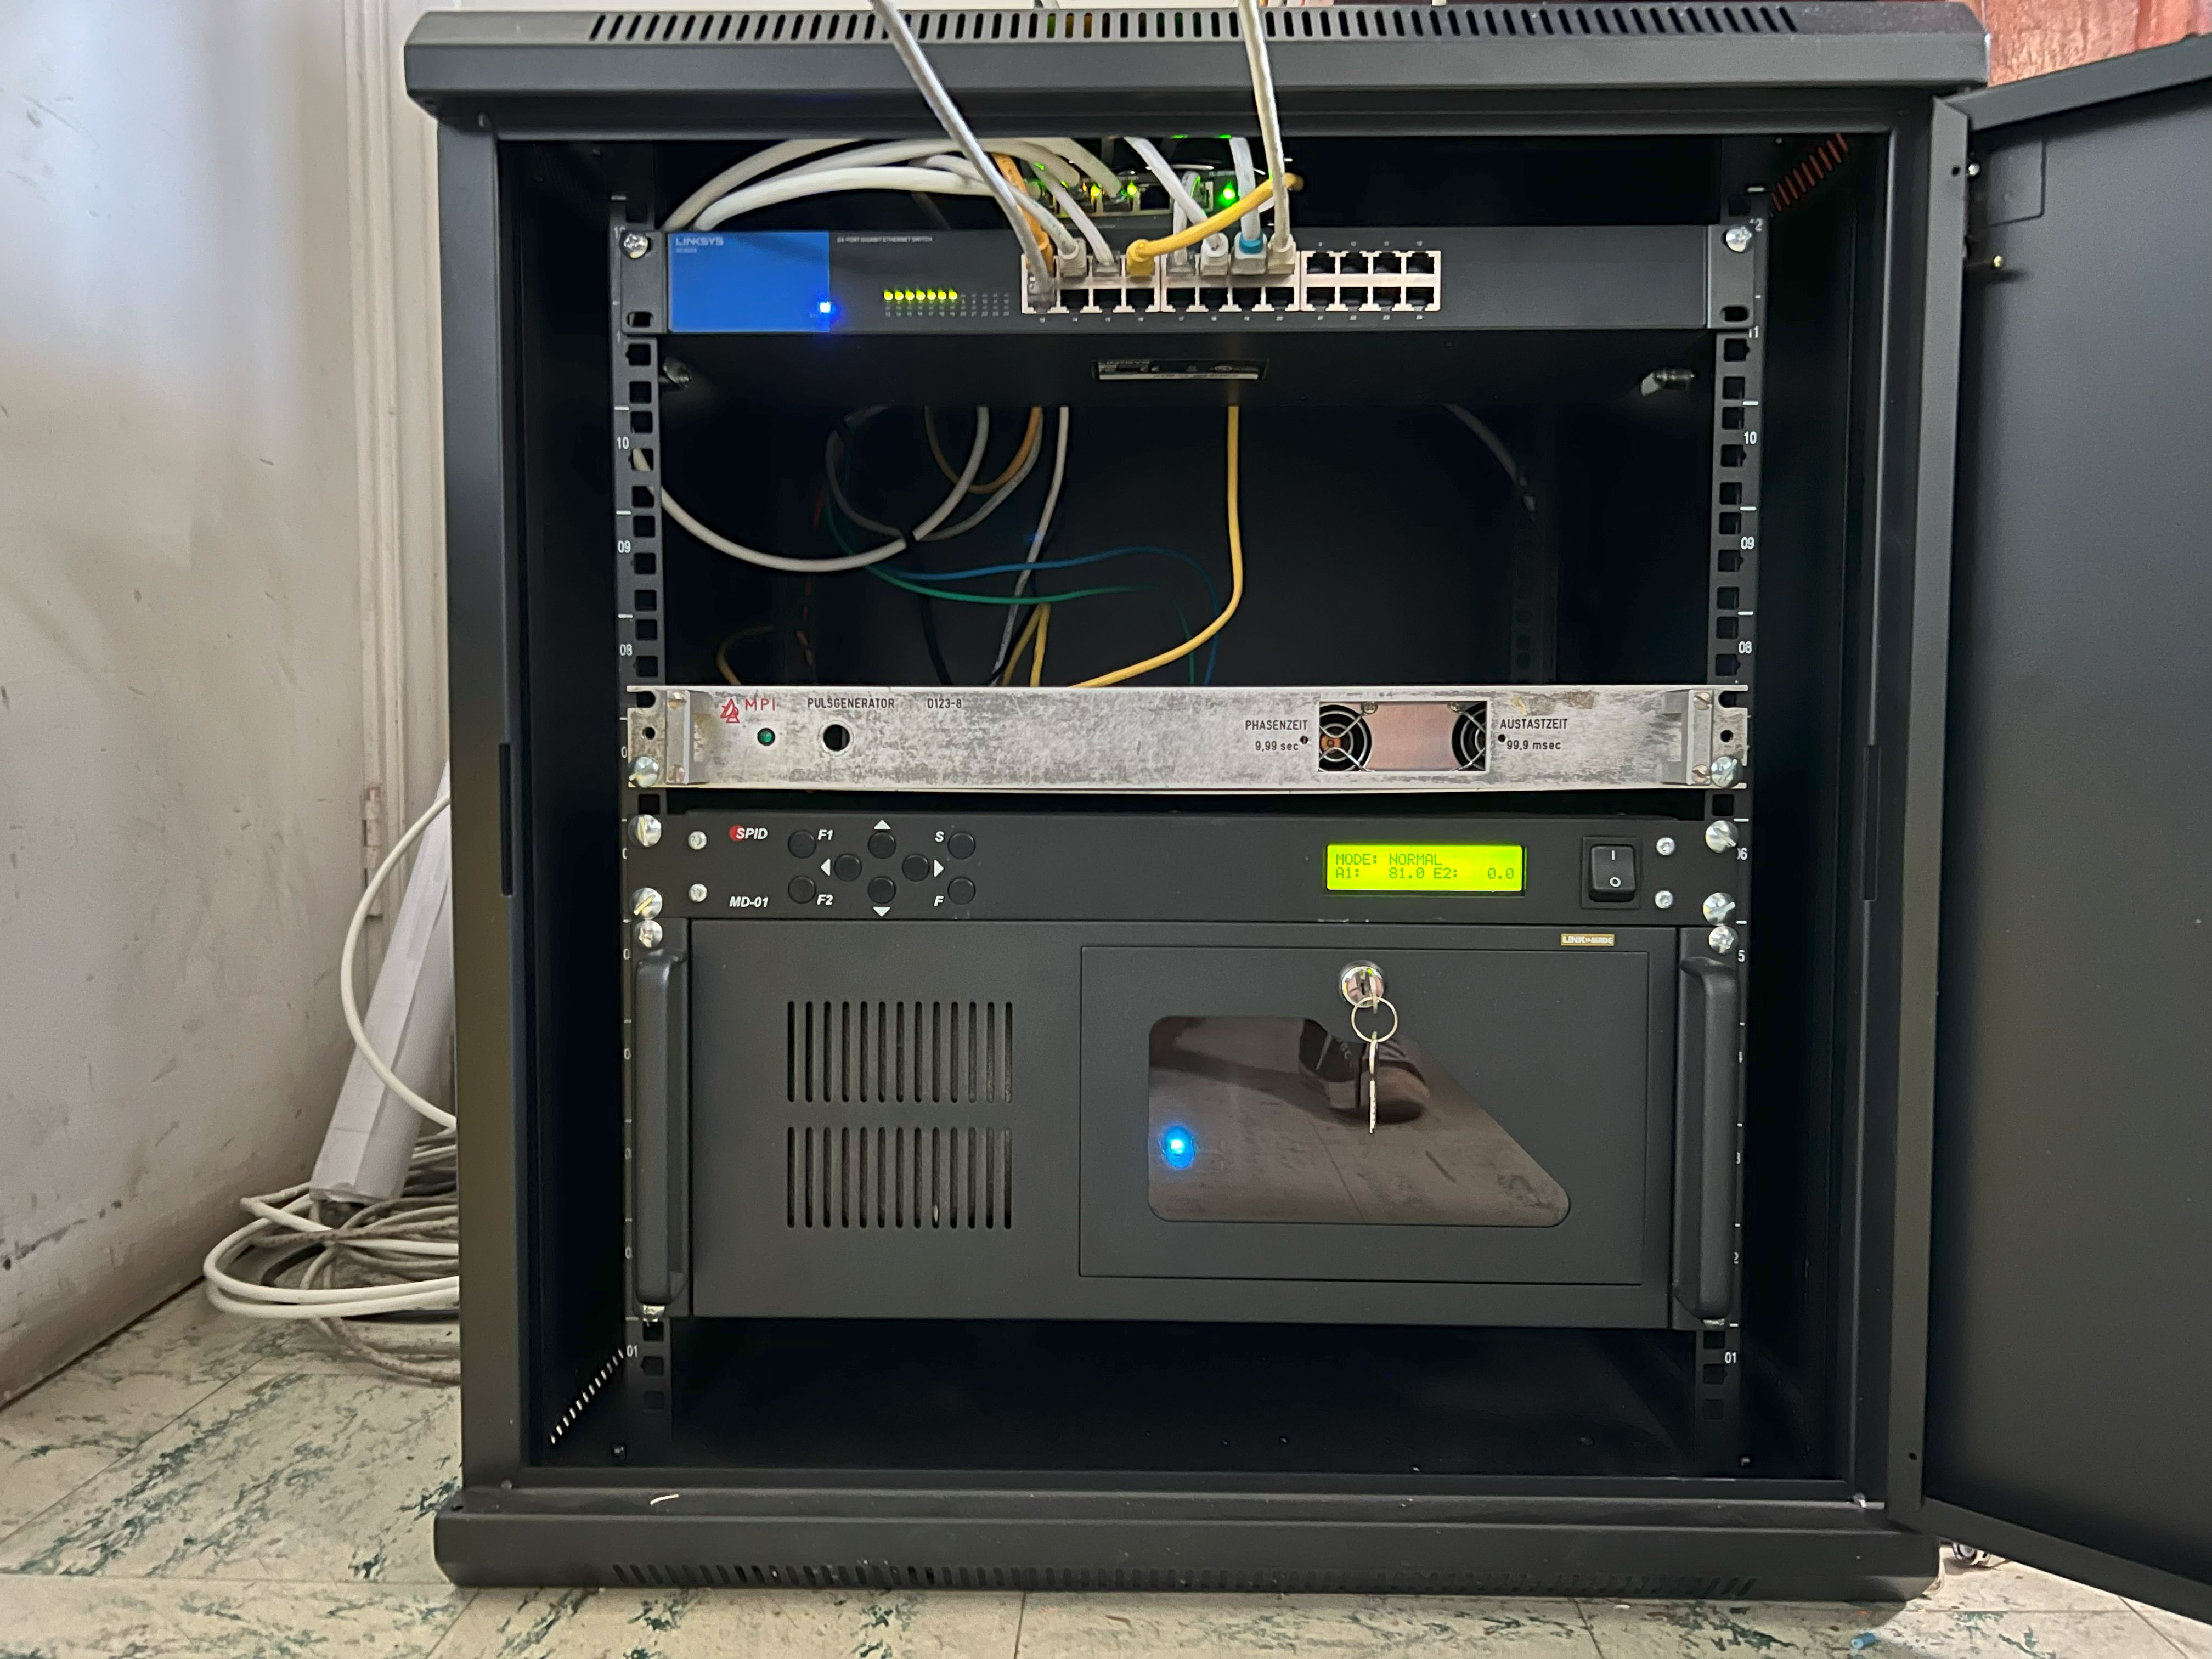
\includegraphics[width=0.8\textwidth]{img/rack}
    \caption{Rack de control con el controlador SPID de la montura y el computador de control.}
    \label{fig:ensamble12}
\end{figure}

En la figura \ref{fig:ensamble12} se puede ver el rack de control con los siguientes elementos ordenados verticalmente: el switch de red, el inyector POE\footnote{Protocolo de energización por cables ethernet con su sigla en inglés, POE\textit{Power Over Ethernet}} del receptor, la fuente de alimentación múltiple, el controlador de la montura SPID, el computador de control y observación. Estos elementos se encuentran en la sala de recepción de ARTE que cuenta con un sistema de climatización que mantiene la temperatura constante a 16 grados Celsius.\\

\section{Alimentador}

Para el alimentador se evaluaron distintas opciones de antenas según su desempeño de ganancia y ancho de banda. Las frecuencias de operación del telescopio son de 1420 MHz para la banda de hidrógeno y de 300 a 500 MHz para la banda de CHARTS.\\

Como una de las características de la construcción del telescopio es la capacidad de intercambiar su alimentador con la estandarización de los soportes, se decidió utilizar antenas comerciales que cumplieran con los requerimientos de operación y se acercaran al rendimiento que declara el fabricante para esta superficie.\\

\subsection{LPDA de alto ancho de banda}

La antena log-periódica de dipolo (LPDA) de alto ancho de banda es una antena que se caracteriza por tener una ganancia de 10 dBi y un ancho de banda de 300 a 6000 MHz. Esta antena se instaló con el elemento más pequeño del arreglo de dipolos en el foco de la parábola. Se orientó con la cara plana de la antena perpendicular con el plano del suelo.\\ 

\begin{figure}
    \centering
    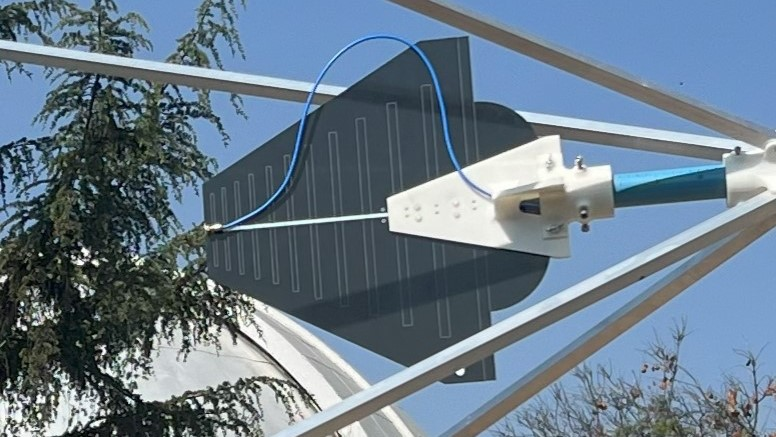
\includegraphics[width=0.8\textwidth]{img/lpda}
    \caption{Antena LPDA de alto ancho de banda instalada en el telescopio.}
    \label{fig:ensamble13}
\end{figure}

La antena de la figura \ref{fig:ensamble13} se instaló en el soporte de la figura \ref{fig:ensamble8} y se conectó al receptor por medio de un cable coaxial de 50 ohmios y 1.5 metros de longitud.\\

\subsection{Dipolo de ARTE}

El dipolo de ARTE es una antena que forma el arreglo del telescopio ARTE \cite{Gallardo2023} esta antena se caracteriza por tener un ancho de banda de 400 MHz desde 1000 para el diseño impreso instalado en el telescopio. Esta antena tiene una ganancia de 3 dBi y se ubica en el foco de la parábola a 135 cm de la superficie.\\

\begin{figure}
    \centering
    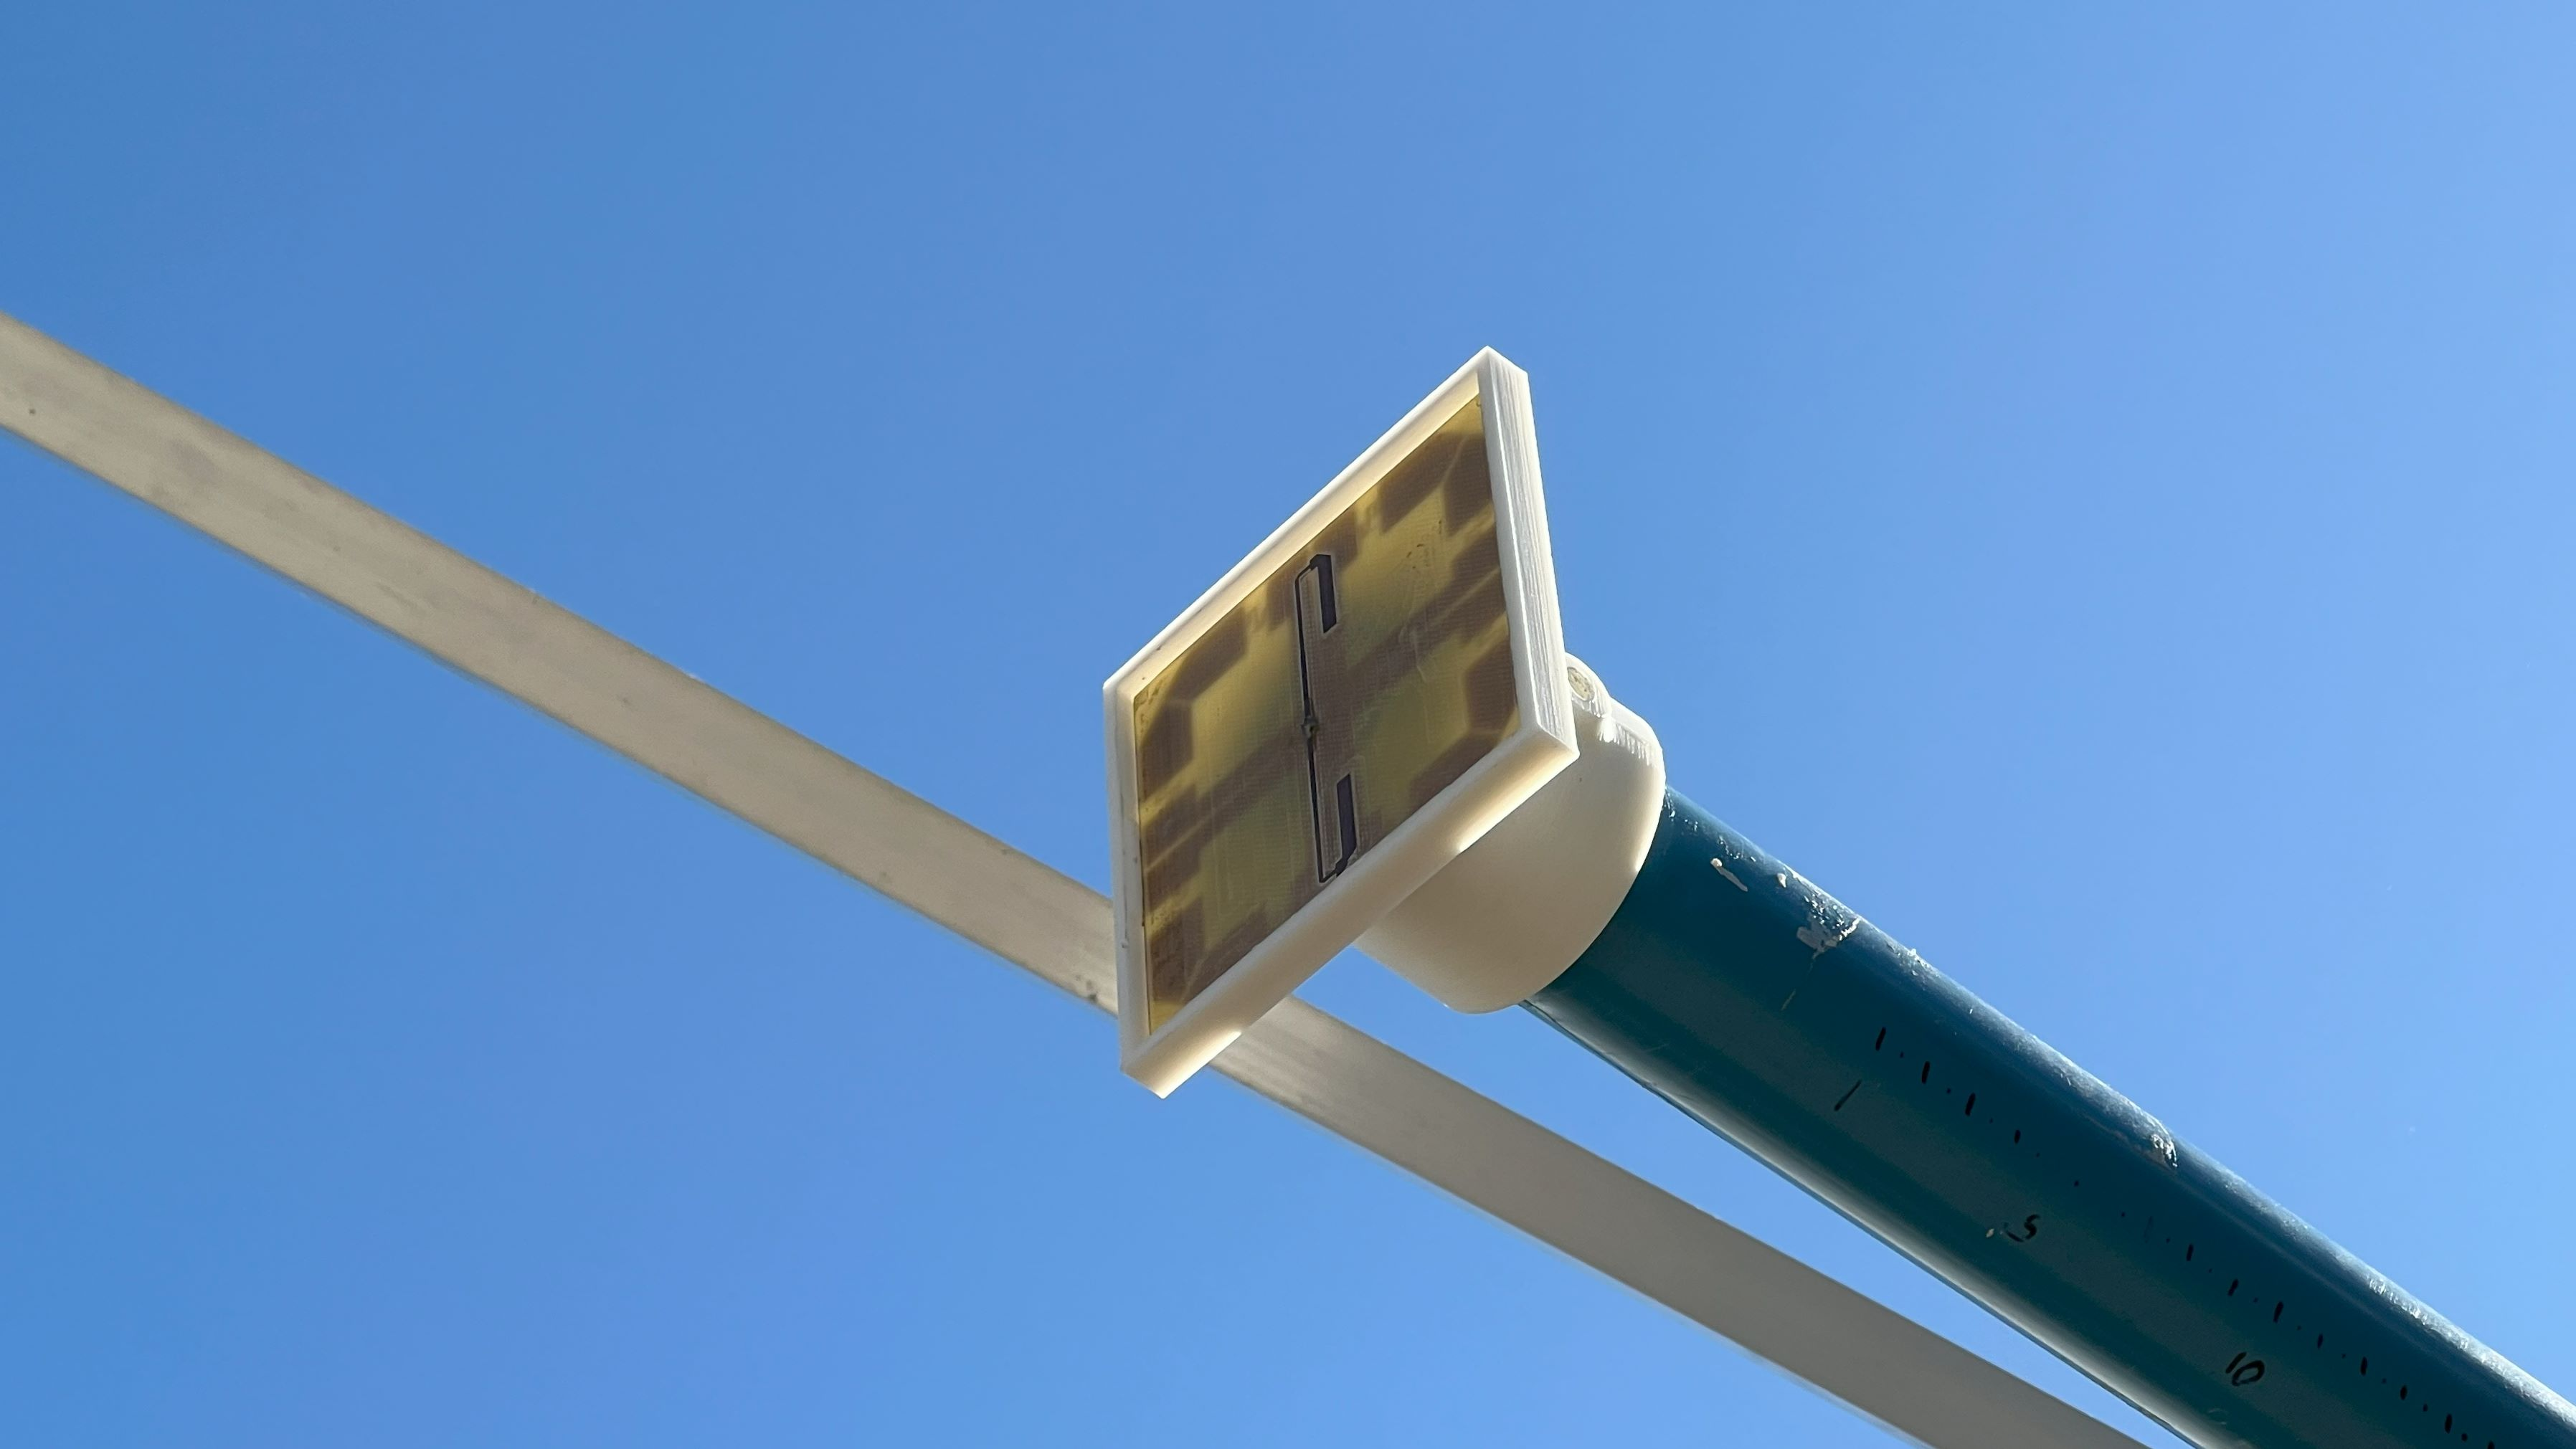
\includegraphics[width=0.8\textwidth]{img/feed}
    \caption{Dipolo de ARTE instalado en el telescopio.}
    \label{fig:ensamble14}
\end{figure}

Esta antena tiene la particularidad de que tiene la ganancia recomendada por el fabricante del reflector para utilizar como alimentador a la distancia de 135 cm. Como se puede ver en la figura \ref{fig:ensamble14} la antena de PCB se encuentra instalada en el tubo de PVC con el soporte diseñado de la figura \ref{fig:ensamble9}.\\

\subsection{Antena circular de alto ancho de banda}

Esta antena es la misma que la utilizada en la fuente de calibración de la copa de agua, en este caso se quiso utilizar como alimentador en reemplazo de la LPDA de la figura \ref{fig:ensamble13}. Esta antena tiene una ganancia cercana a 3 dBi, semejante a la del dipolo de ARTE y lo que se recomienda para el reflector. La antena se instala en el soporte de la figura \ref{fig:ensamble7}.\\

\begin{figure}
    \centering
    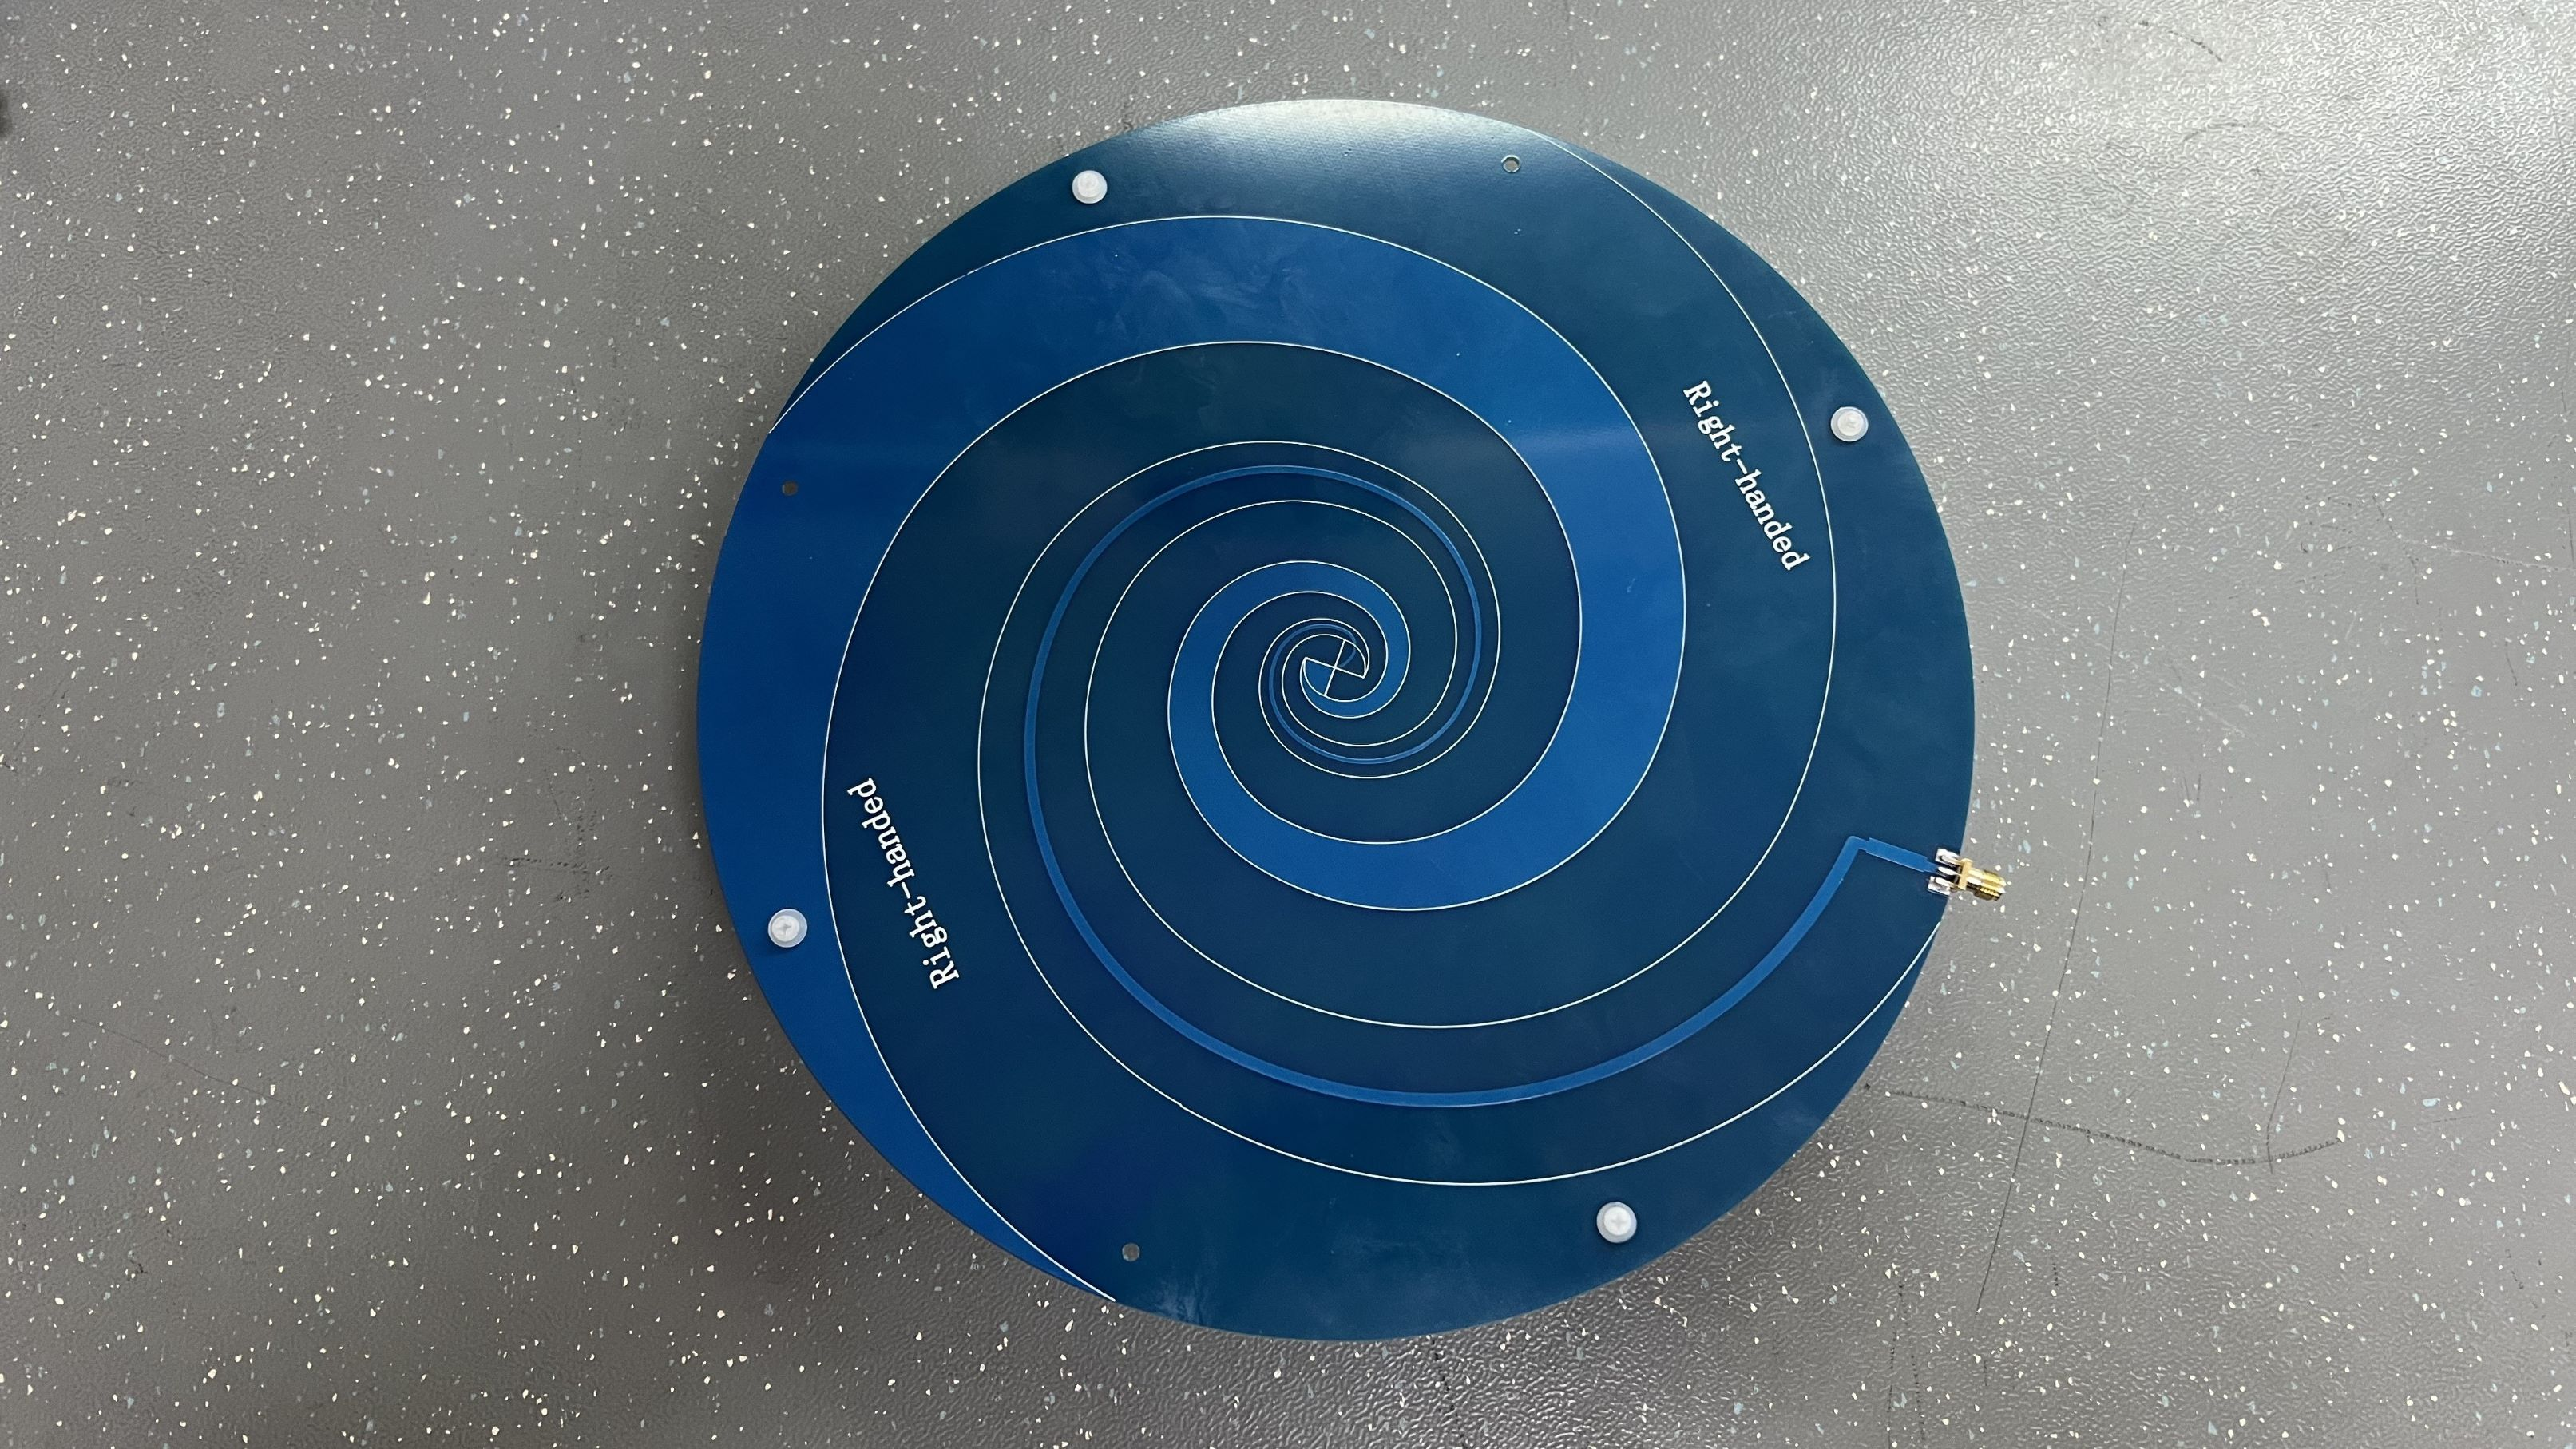
\includegraphics[width=0.8\textwidth]{img/paletaFeed}
    \caption{Antena circular de alto ancho de banda instalada en el telescopio.}
    \label{fig:ensamble15}
\end{figure}


\section{Diseño del receptor}

Para el receptor se optó por utilizar una SDR de bajo costo, un filtro pasabanda optimizado para la observación de la banda de hidrógeno y un amplificador de bajo ruido. Se tomó en cuenta que estos componentes deben no solo ser de alta precisión, sino que también robustos, ya que estarán ubicados lo más cerca posible del alimentador a la intemperie.\\

\subsection{Cadena de recepción}

Para la cadena de recepción cuenta con un empaquetado de un amplificador de bajo ruido de la compañía \textit{Noeelec} que contiene además un filtro pasabanda de 75 MHz de ancho de banda centrado en 1420 MHz. El amplificador tiene una ganancia típica a 1.4 GHz de 35 dB con una figura de ruido de 0.6 dB para la misma frecuencia. Además, este amplificador puede ser alimentado por bias-tee\footnote{Circuitos de inyección de corriente continua a travez de líneas coaxiales de RF} desde la misma SDR.\\

\begin{figure}
    \centering
    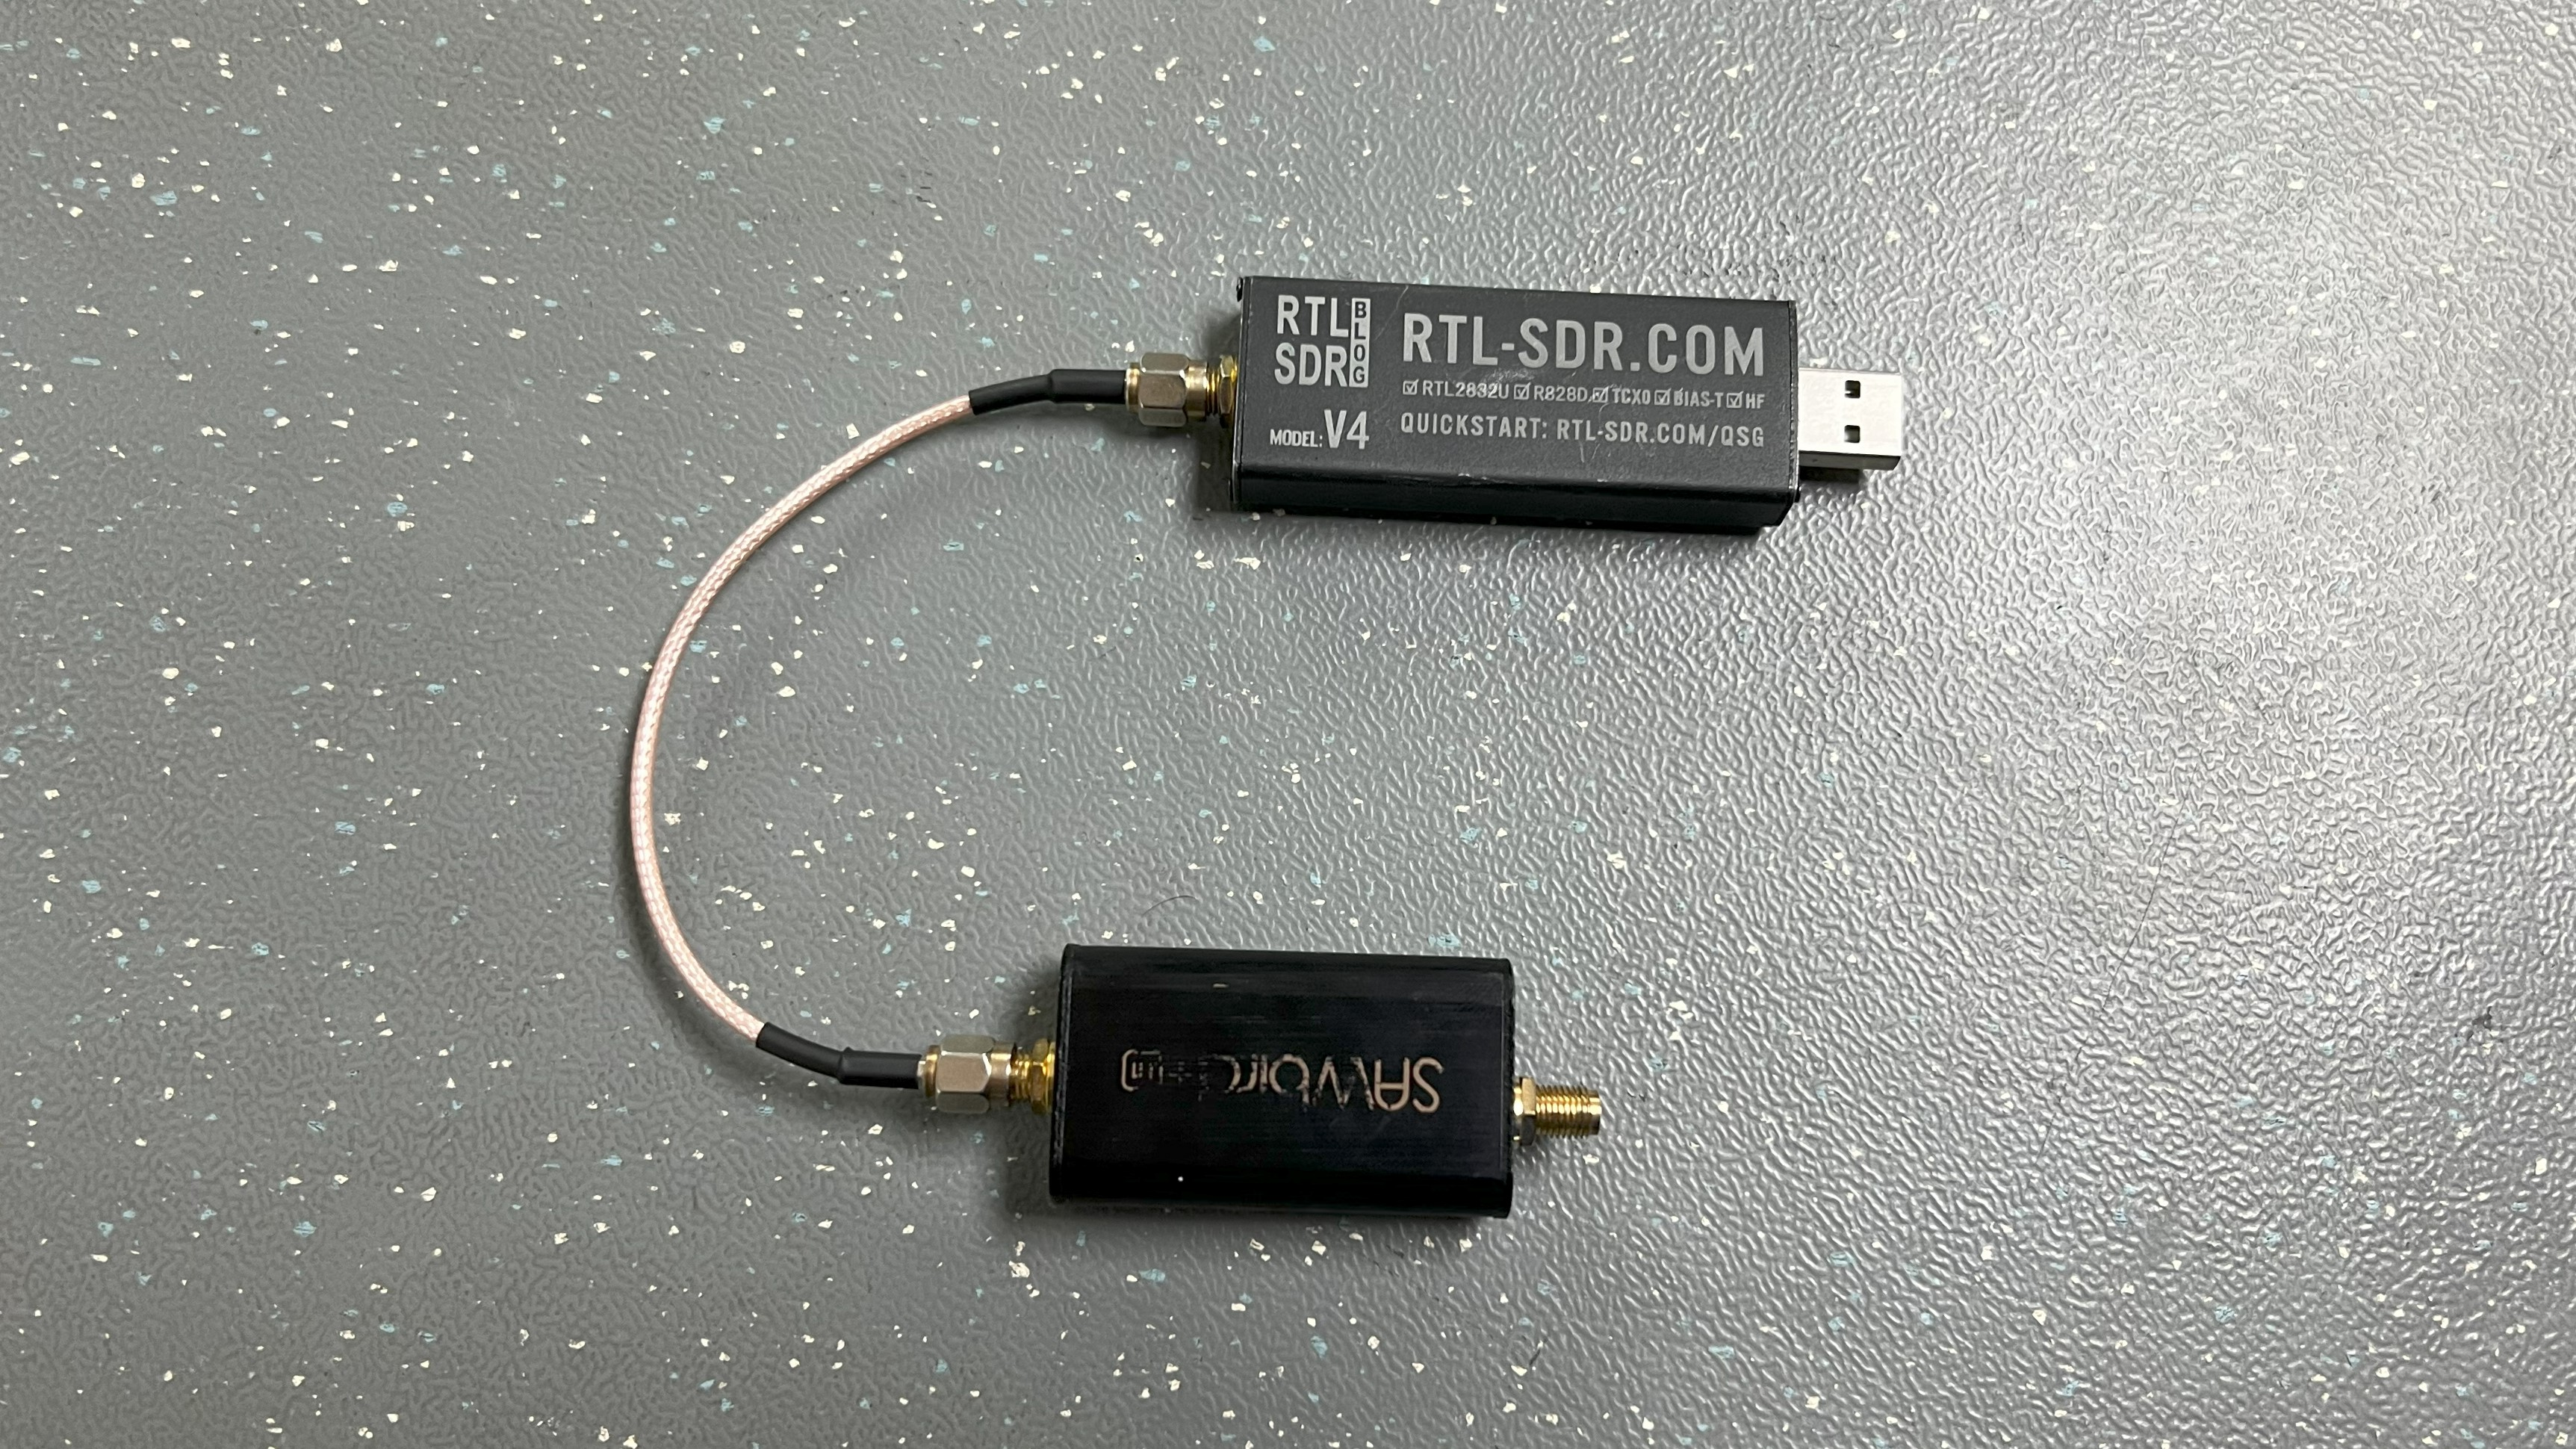
\includegraphics[width=0.8\textwidth]{img/rtl_saw}
    \caption{Amplificador y filtro pasabanda SAWbird H1 de la compañía \textit{Noeelec}.}
    \label{fig:cadena}
\end{figure}

En la figura \ref{fig:cadena} se puede ver el amplificador y filtro pasabanda SAWbird H1 de la compañía conectado a un analizador de espectro y una fuente de ruido para la caracterización de la cadena de recepción.\\

\subsection{Digitalizador y adquisición}

El digitalizador es una RTL-SDR de la organización \textit{RTL-SDR} basado en el chip R820T de \textit{Rafael Micro} que se conecta por USB a un computador para obtener directamente el voltaje complejo de la IF para que sea procesada por el software de adquisición. Este digitalizador tiene una frecuencia de muestreo máxima de 3.2 MS/s y una resolución de 8 bits, pero usualmente se utiliza bajo los 2.56 MS/s para que tenga un comportamiento estable \cite{RTLSDR2018}.\\

\begin{figure}
    \centering
    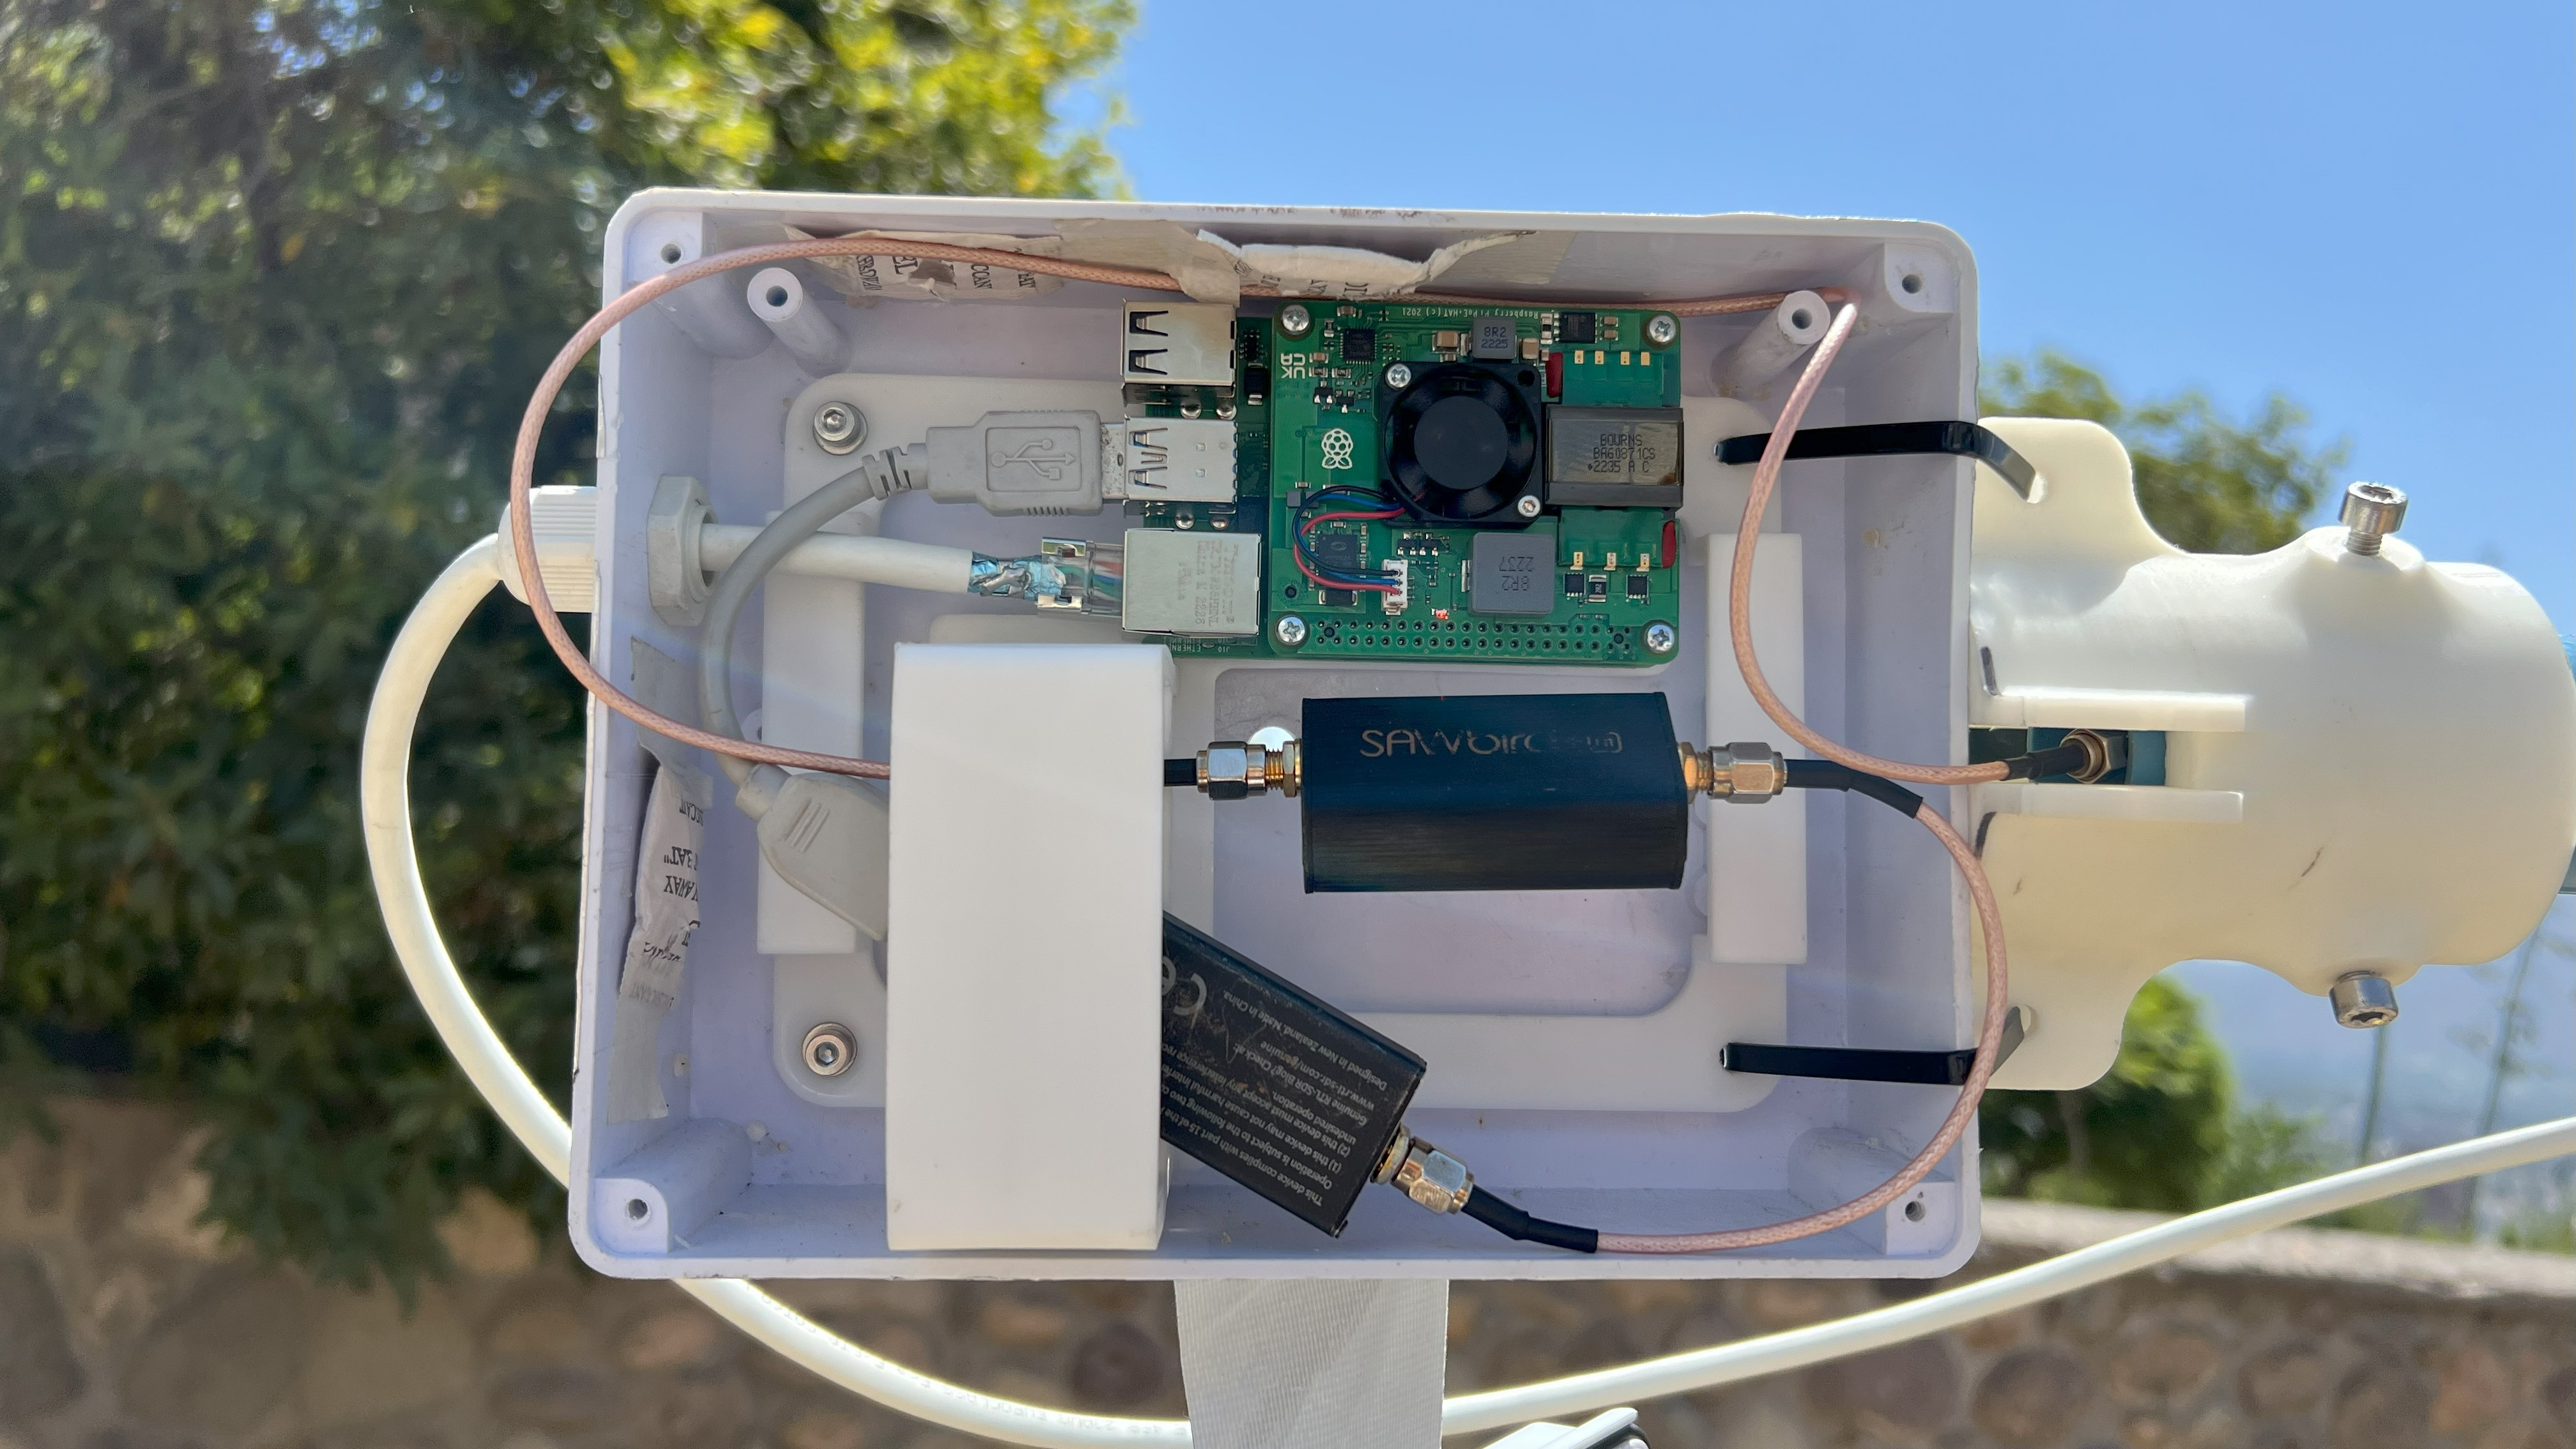
\includegraphics[width=0.8\textwidth]{img/rpiRtlSaw}
    \caption{RTL-SDR conectada a la cadena de amplificador y una Raspberry PI 4B.}
    \label{fig:digitalizador}
\end{figure}

En la figura \ref{fig:digitalizador} se puede ver la RTL-SDR conectada a la cadena de amplificador y una Raspberry PI 4B con un \textit{Hat} POE. Se utilizó esta configuración para llevar solo un cable ethernet cat 6 por el cual pasaría la energía y los datos. La Raspberry es capaz de alimentar a la SDR que a su vez por medio de su Bias-Tee puede alimentar al amplificador de bajo ruido con la mínima cantidad posible de cables y conexiones.\\

El cable ethernet utilizado es un cat 6 de 25 metros, que va desde el receptor al rack de control. Este cable es del tipo FFTP, lo que quiere decir que cada par trenzado está recubierto con una lámina de aluminio y a su vez los 4 pares trenzados más un conductor de apantallamiento están recubiertos por otra lámina de aluminio que se conecta a tierra en ambos extremos para minimizar el ruido al transportar datos y no producir RFI al telescopio.\\

\section{Software de control y adquisición} \label{sec:software}

La infraestructura digital del telescopio se diseñó con un factor principal en mente, que este se pueda operar completamente remoto, por lo que todo el software está hecho para ser operado desde cualquier lugar con acceso a internet. Accediendo a la terminal de control por medio de SSH\footnote{SSH del inglés Secure Shell, es un protocolo de envío de comandos a un computador de forma segura.} y todos sus sistemas están conectados a una red local por medio de ethernet.\\

El principal lenguaje de programación utilizado para el desarrollo de software fue python, por su simplicidad a la hora de generar entornos virtuales de desarrollo y librerías existentes para utilizar los diversos subsistemas, como por ejemplo, el uso de la librería de \textit{astropy} para los cálculos de seguimiento.\\

\subsection{Control de la montura}

El controlador del rotor requiere una comunicación específica en hexagesimal para moverse y a través del mismo protocolo responde con la posición en la cual se encuentra. Para esto se creó una librería en python basada en el protocolo Rot2Prog \cite{rot2prog} que empaqueta y traduce los comandos de movimiento, elevación y azimuth. Esta librería es un archivo de python por el nombre de spid.py, la que es importada para todos los demás códigos de control.\\

\paragraph{control.py} Es el código principal de control, tiene la capacidad de mandar una posición de azimuth y elevación, de pedir la posición actual de la montura, de reiniciar el controlador en caso de que no responda a los comandos y una de las funciones más importantes es el parado de emergencia de cualquier movimiento.\\

\paragraph{cpt\_traking\_software.py} Este es un software más sofisticado que se creó para el seguimiento de cuerpos celestes. A partir de las coordenadas de declinación y ascensión recta, el software calcula la posición de la montura para este astro según la ubicación del telescopio y la hora local.\\

\begin{figure}
    \centering
    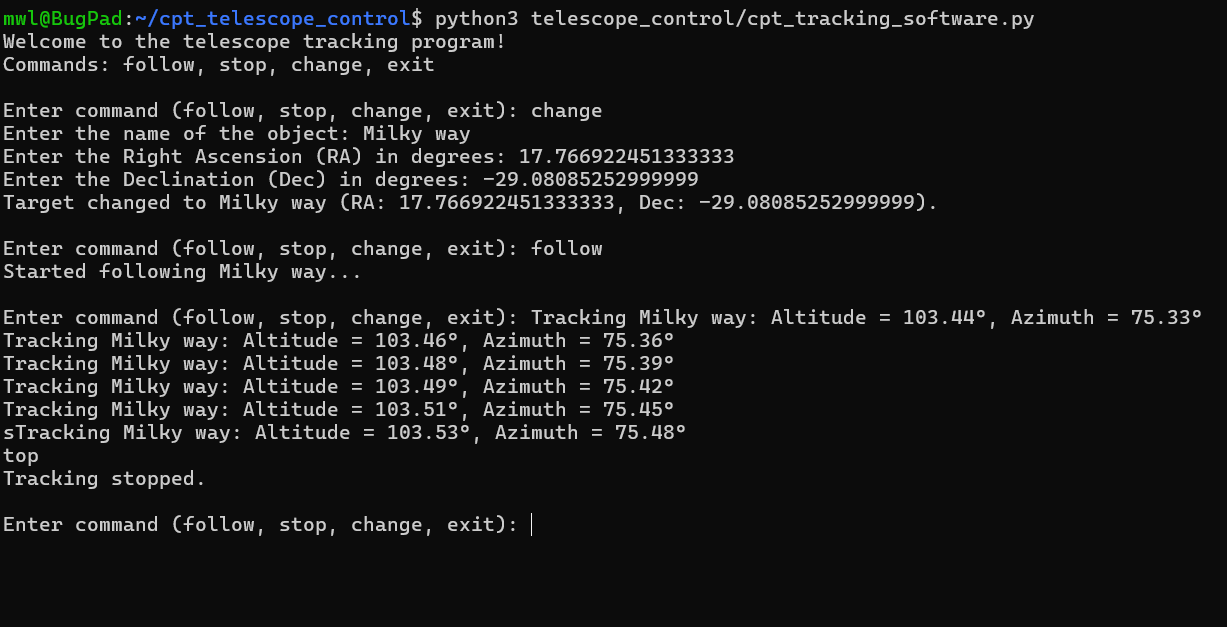
\includegraphics[width=0.8\textwidth]{img/traking}
    \caption{cpt\_traking\_software.py en funcionamiento.}
    \label{fig:control}
\end{figure}

En la figura \ref{fig:control} se puede ver el software en funcionamiento, con las opciones de cambiar el objeto a seguir \textit{change}, el seguimiento del objeto \textit{follow} y el parado del movimiento \textit{stop}. El software es capaz de invertir la posición de elevación del telescopio para minimizar el movimiento en azimut y evitar que los cables puedan enrollarse entre sí.\\

Por ejemplo, si al calcular que la posición del astro en elevación de 50 grados y azimuth de 315, requiere un movimiento de más de 180 grados en azimut, el software invierte la posición de elevación para que el movimiento sea menor a 180 grados resultando en que el telescopio apunte a 130 grados de elevación y a 135 grados en azimut. De forma automática, si el astro tiene una elevación menor a los 30 grados, o mayor a 150 grados en la inversión, este deja de seguir el astro ya que a esta elevación la interferencia de radio es muy notoria.\\

\subsection{Adquisición de datos} 

Para la adquisición de datos se crearon 2 softwares en python para esta tarea, uno para adquirir una acumulación de espectros para las observaciones de un objeto celeste y otro para la calibración del instrumento.\\

\paragraph{rtl\_spectra.py} Es un script que utiliza la radio RTL-SDR para obtener espectros mediante un comando específico, este se utiliza principalmente para las caracterizaciones y las mediciones. Se usa en conjunto con el software de control para crear las variantes de medición de patrón de radiación. Se puede configurar la taza de datos, el tamaño de la FFT, la cantidad de espectros tomados y el formato de guardado.\\

\paragraph{cpt\_rtl\_adquisition.py} Es el software de observación, el cual tiene un \textit{Ring buffer} o un acumulador de espectros flotantes, esto quiere decir que, según como se configure, puede acumular una cantidad de espectros que se van actualizando constantemente con nuevos espectros y eliminando los viejos en la ventana de tiempo que se requiera o en lo que la memoria pueda guardar.\\

Al igual que el script anterior este se puede configurar para la tasa de datos, el tamaño de la FFT, la cantidad de espectros tomados y el formato de guardado. Este, por otra parte, está diseñado para obtener una gran cantidad de espectros para ser guardados en una estructura eficiente en espacio en código binario. También tiene la tarea de mostrar en tiempo real la acumulación promediada de los espectros y en paralelo obtener las muestras y agregarlas al ring-buffer.\\


\section{Infraestructura de caracterización}

Para caracterizar el telescopio, se requiere una serie de instrumentos y elementos que permitan obtener los datos necesarios para su calibración y la verificación de los resultados.\\

\subsection{Fuente de calibración}

Ya que el campo lejano de las antenas eléctricamente grandes, como es el caso de una antena de apertura, para medir el patrón de radiación en potencia de una antena se requiere de una fuente de radiofrecuencia conocida a una distancia mayor a la de campo lejano de la antena que se quiere medir.\\

Para esto se instaló una antena de alto ancho de banda (192 MHz a 8 GHz) en la copa de agua del cerro Calán, con un cable coaxial de 20 metros de longitud. Al dejar la antena instalada en la parte superior y pudiéndose instalar generadores de señales desde la parte inferior. A esta antena le llamamos la \quotes{estrella artificial}.\\

\begin{figure}
    \centering
    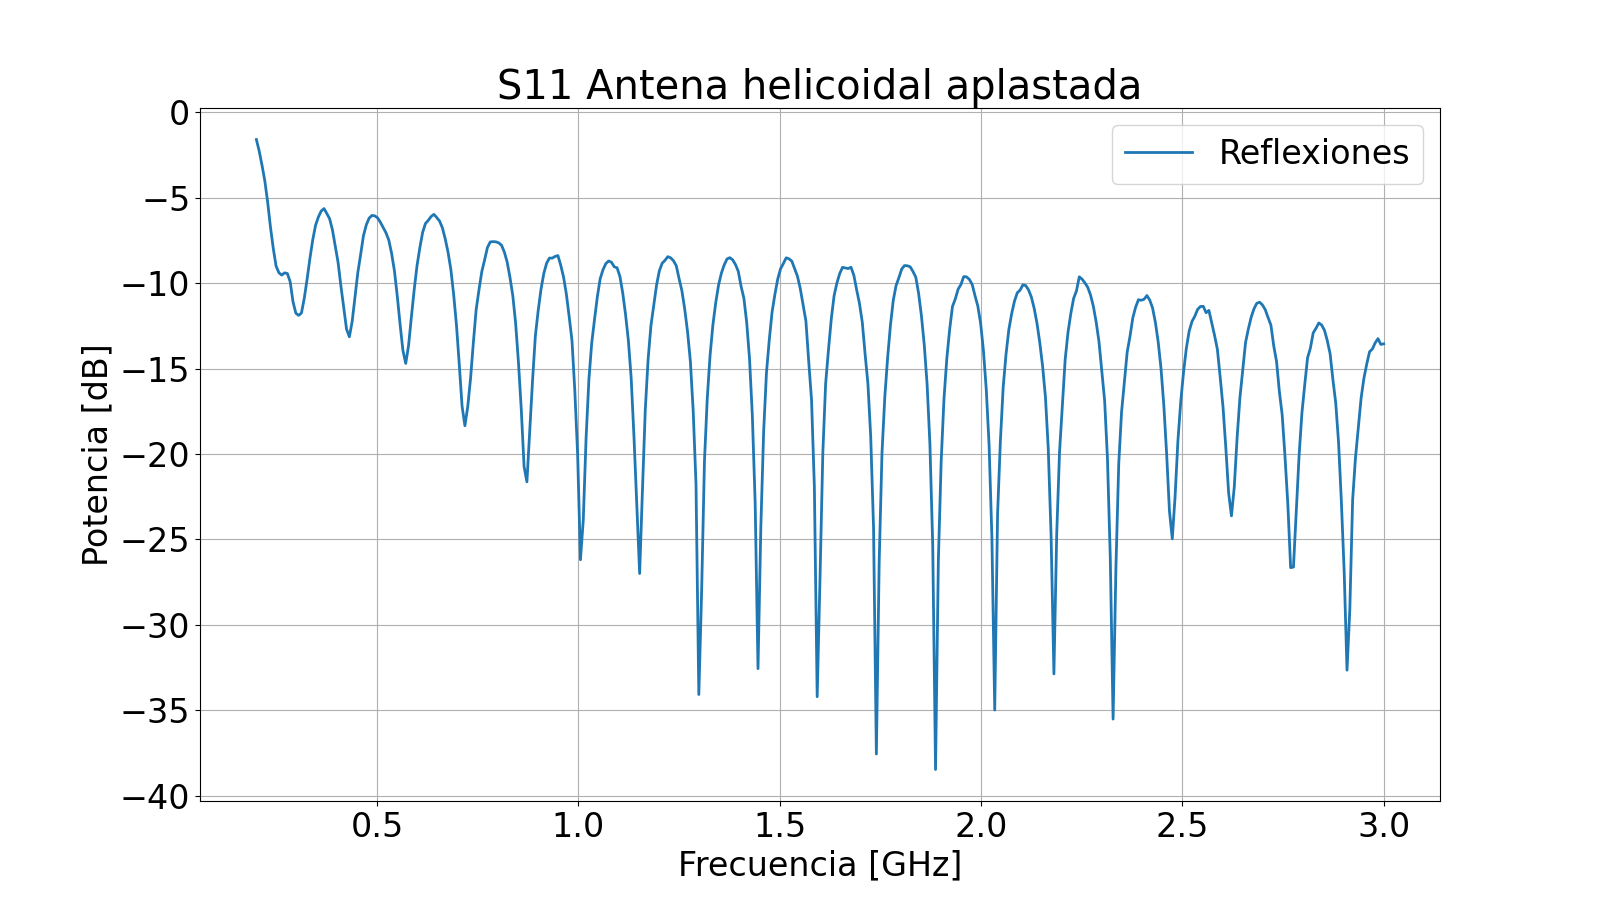
\includegraphics[width=0.8\textwidth]{img/s11Paleta}
    \caption{Parametro S11 para la antena utilizada en la fuente de calibración.}
    \label{fig:s11estrella}
\end{figure}

El ancho de banda de esta antena tiene dos criterios de zona óptima de operación, como se puede apreciar en la figura \ref{fig:s11estrella}, el primer criterio es que la antena posee un ancho de banda bajo los -6 dB de reflexiones para el rango de 192 MHz a 1 GHz y luego para el otro criterio de -10 dB de reflexiones para el rango de 1 GHz a 3 GHz.\\

\begin{figure}[h!]
    \centering
    \begin{subfigure}{0.45\textwidth}
        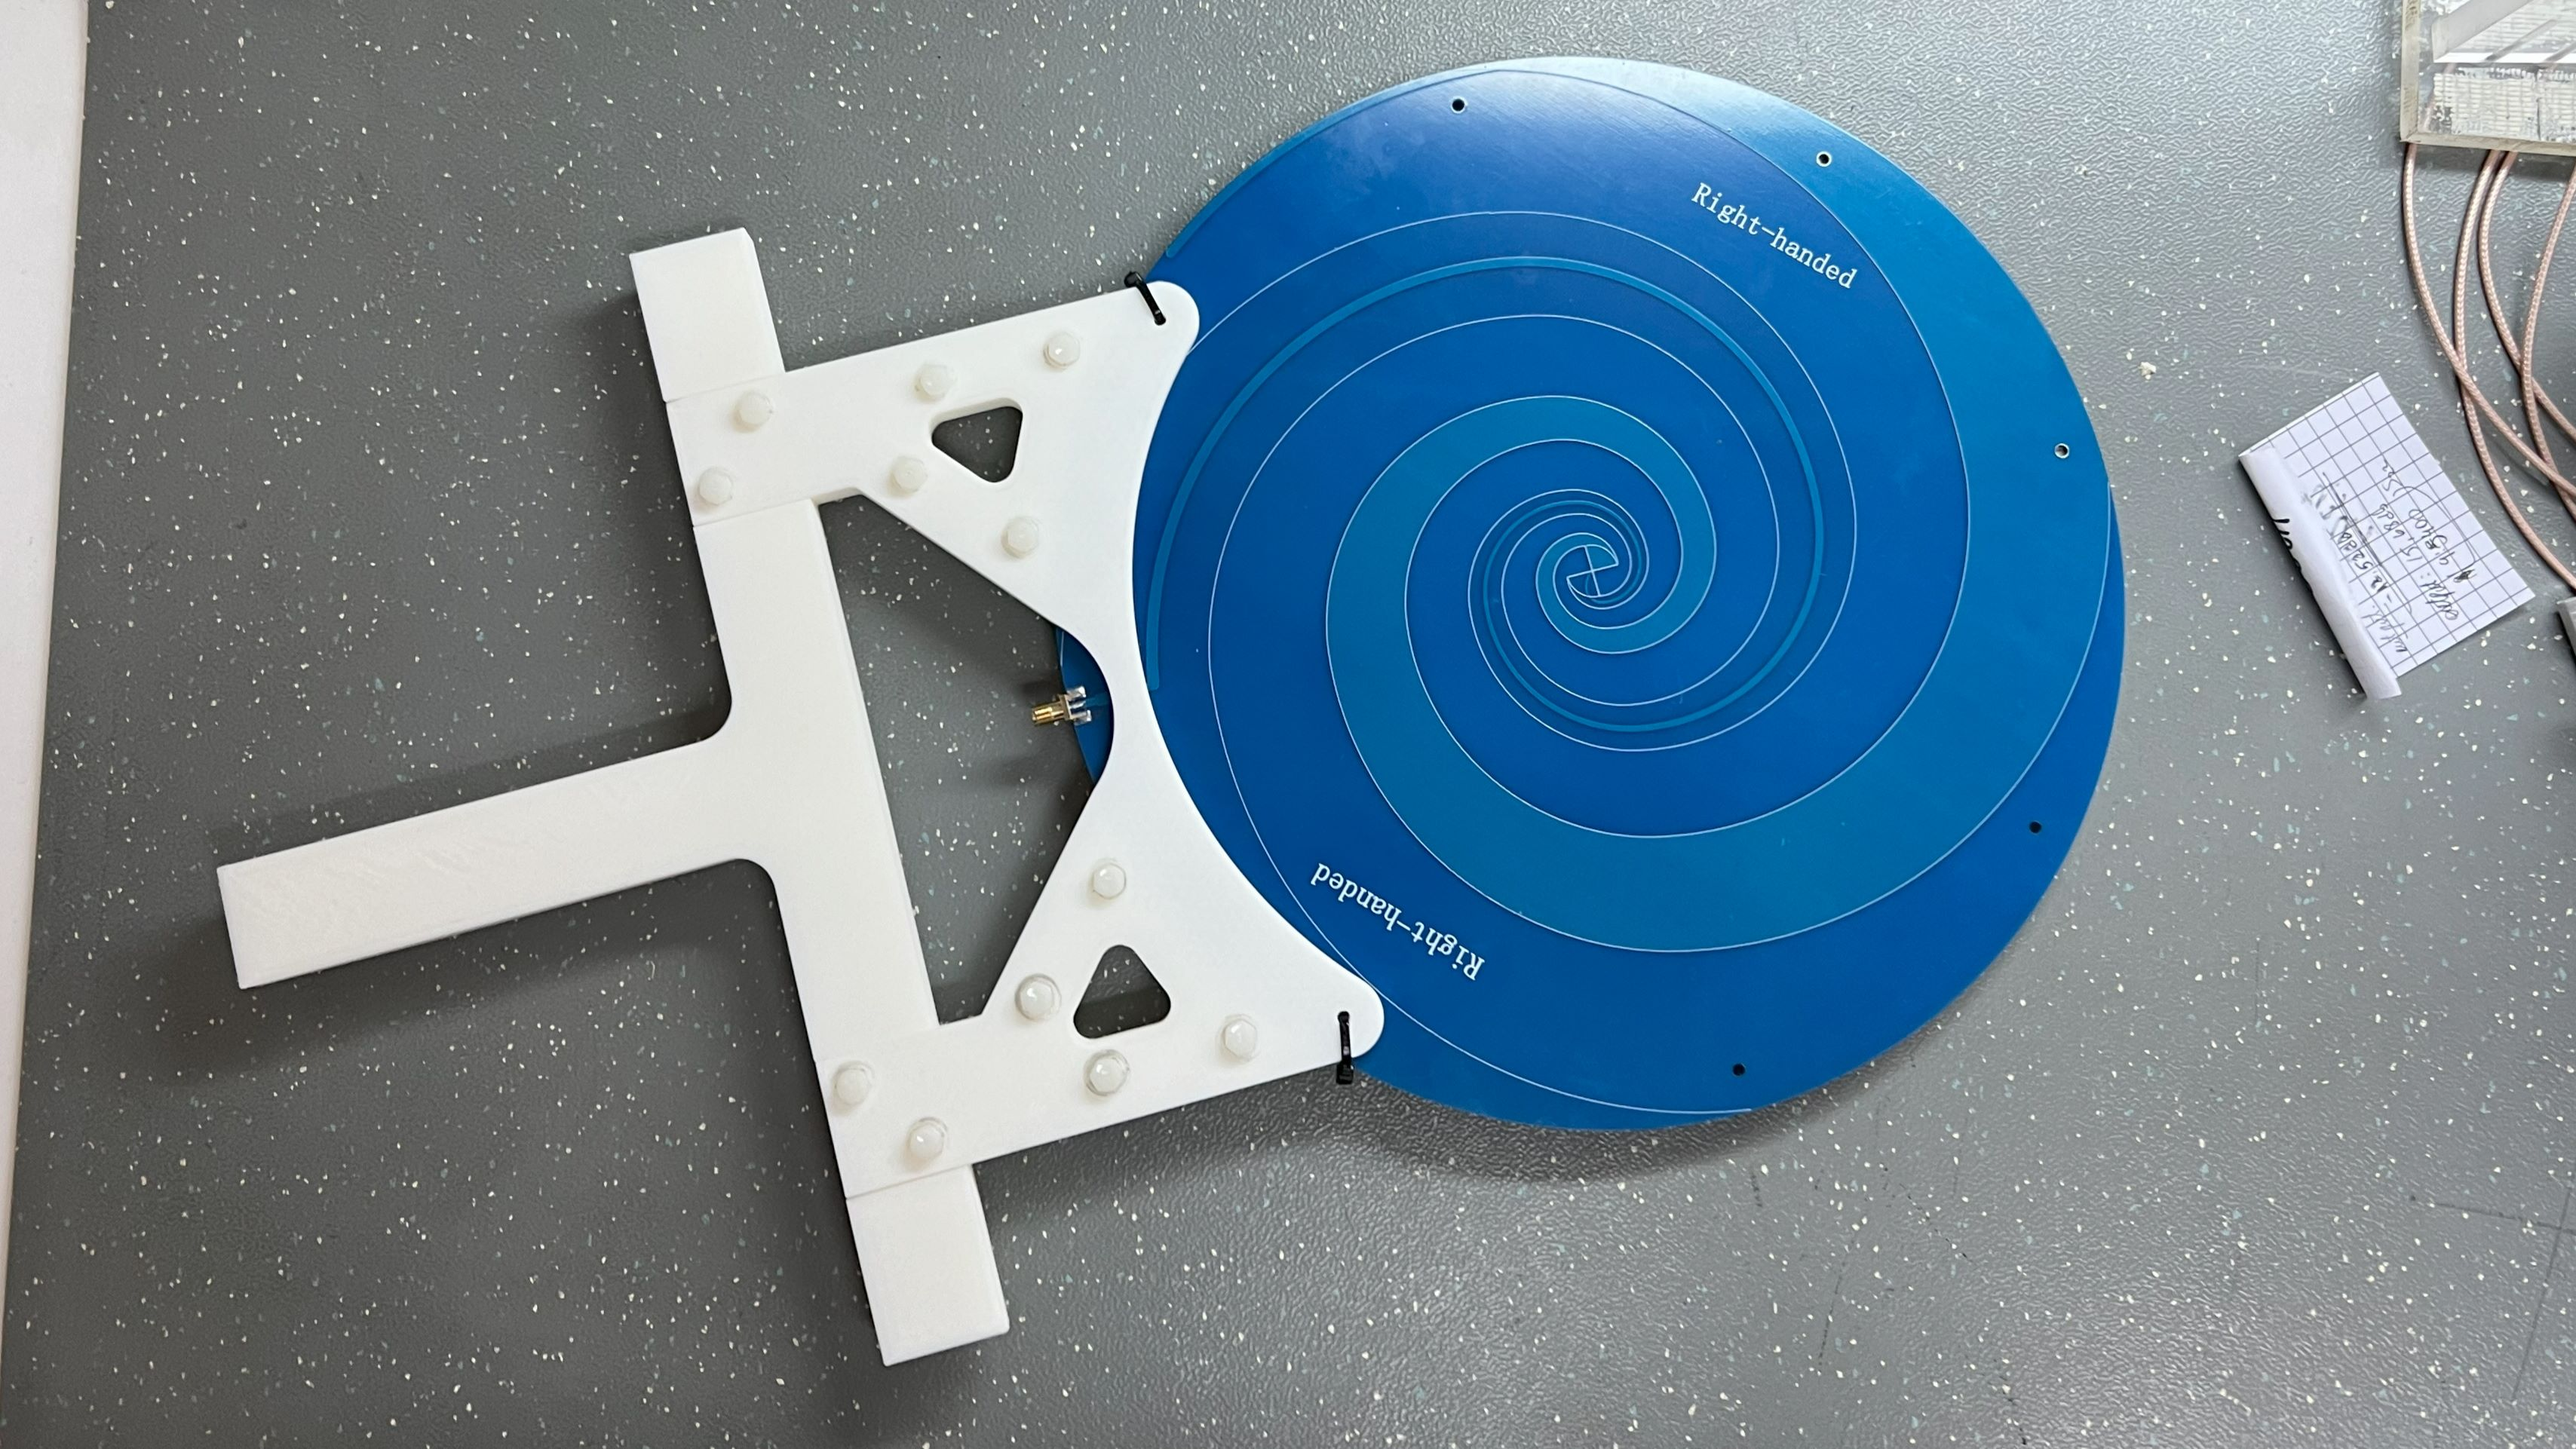
\includegraphics[width=\textwidth]{img/paleta}
        \caption{Antena de polarización circular de alto ancho de banda con su soporte para la copa de agua.}
        \label{fig:antena_estrella}
    \end{subfigure}
    \begin{subfigure}{0.45\textwidth}
        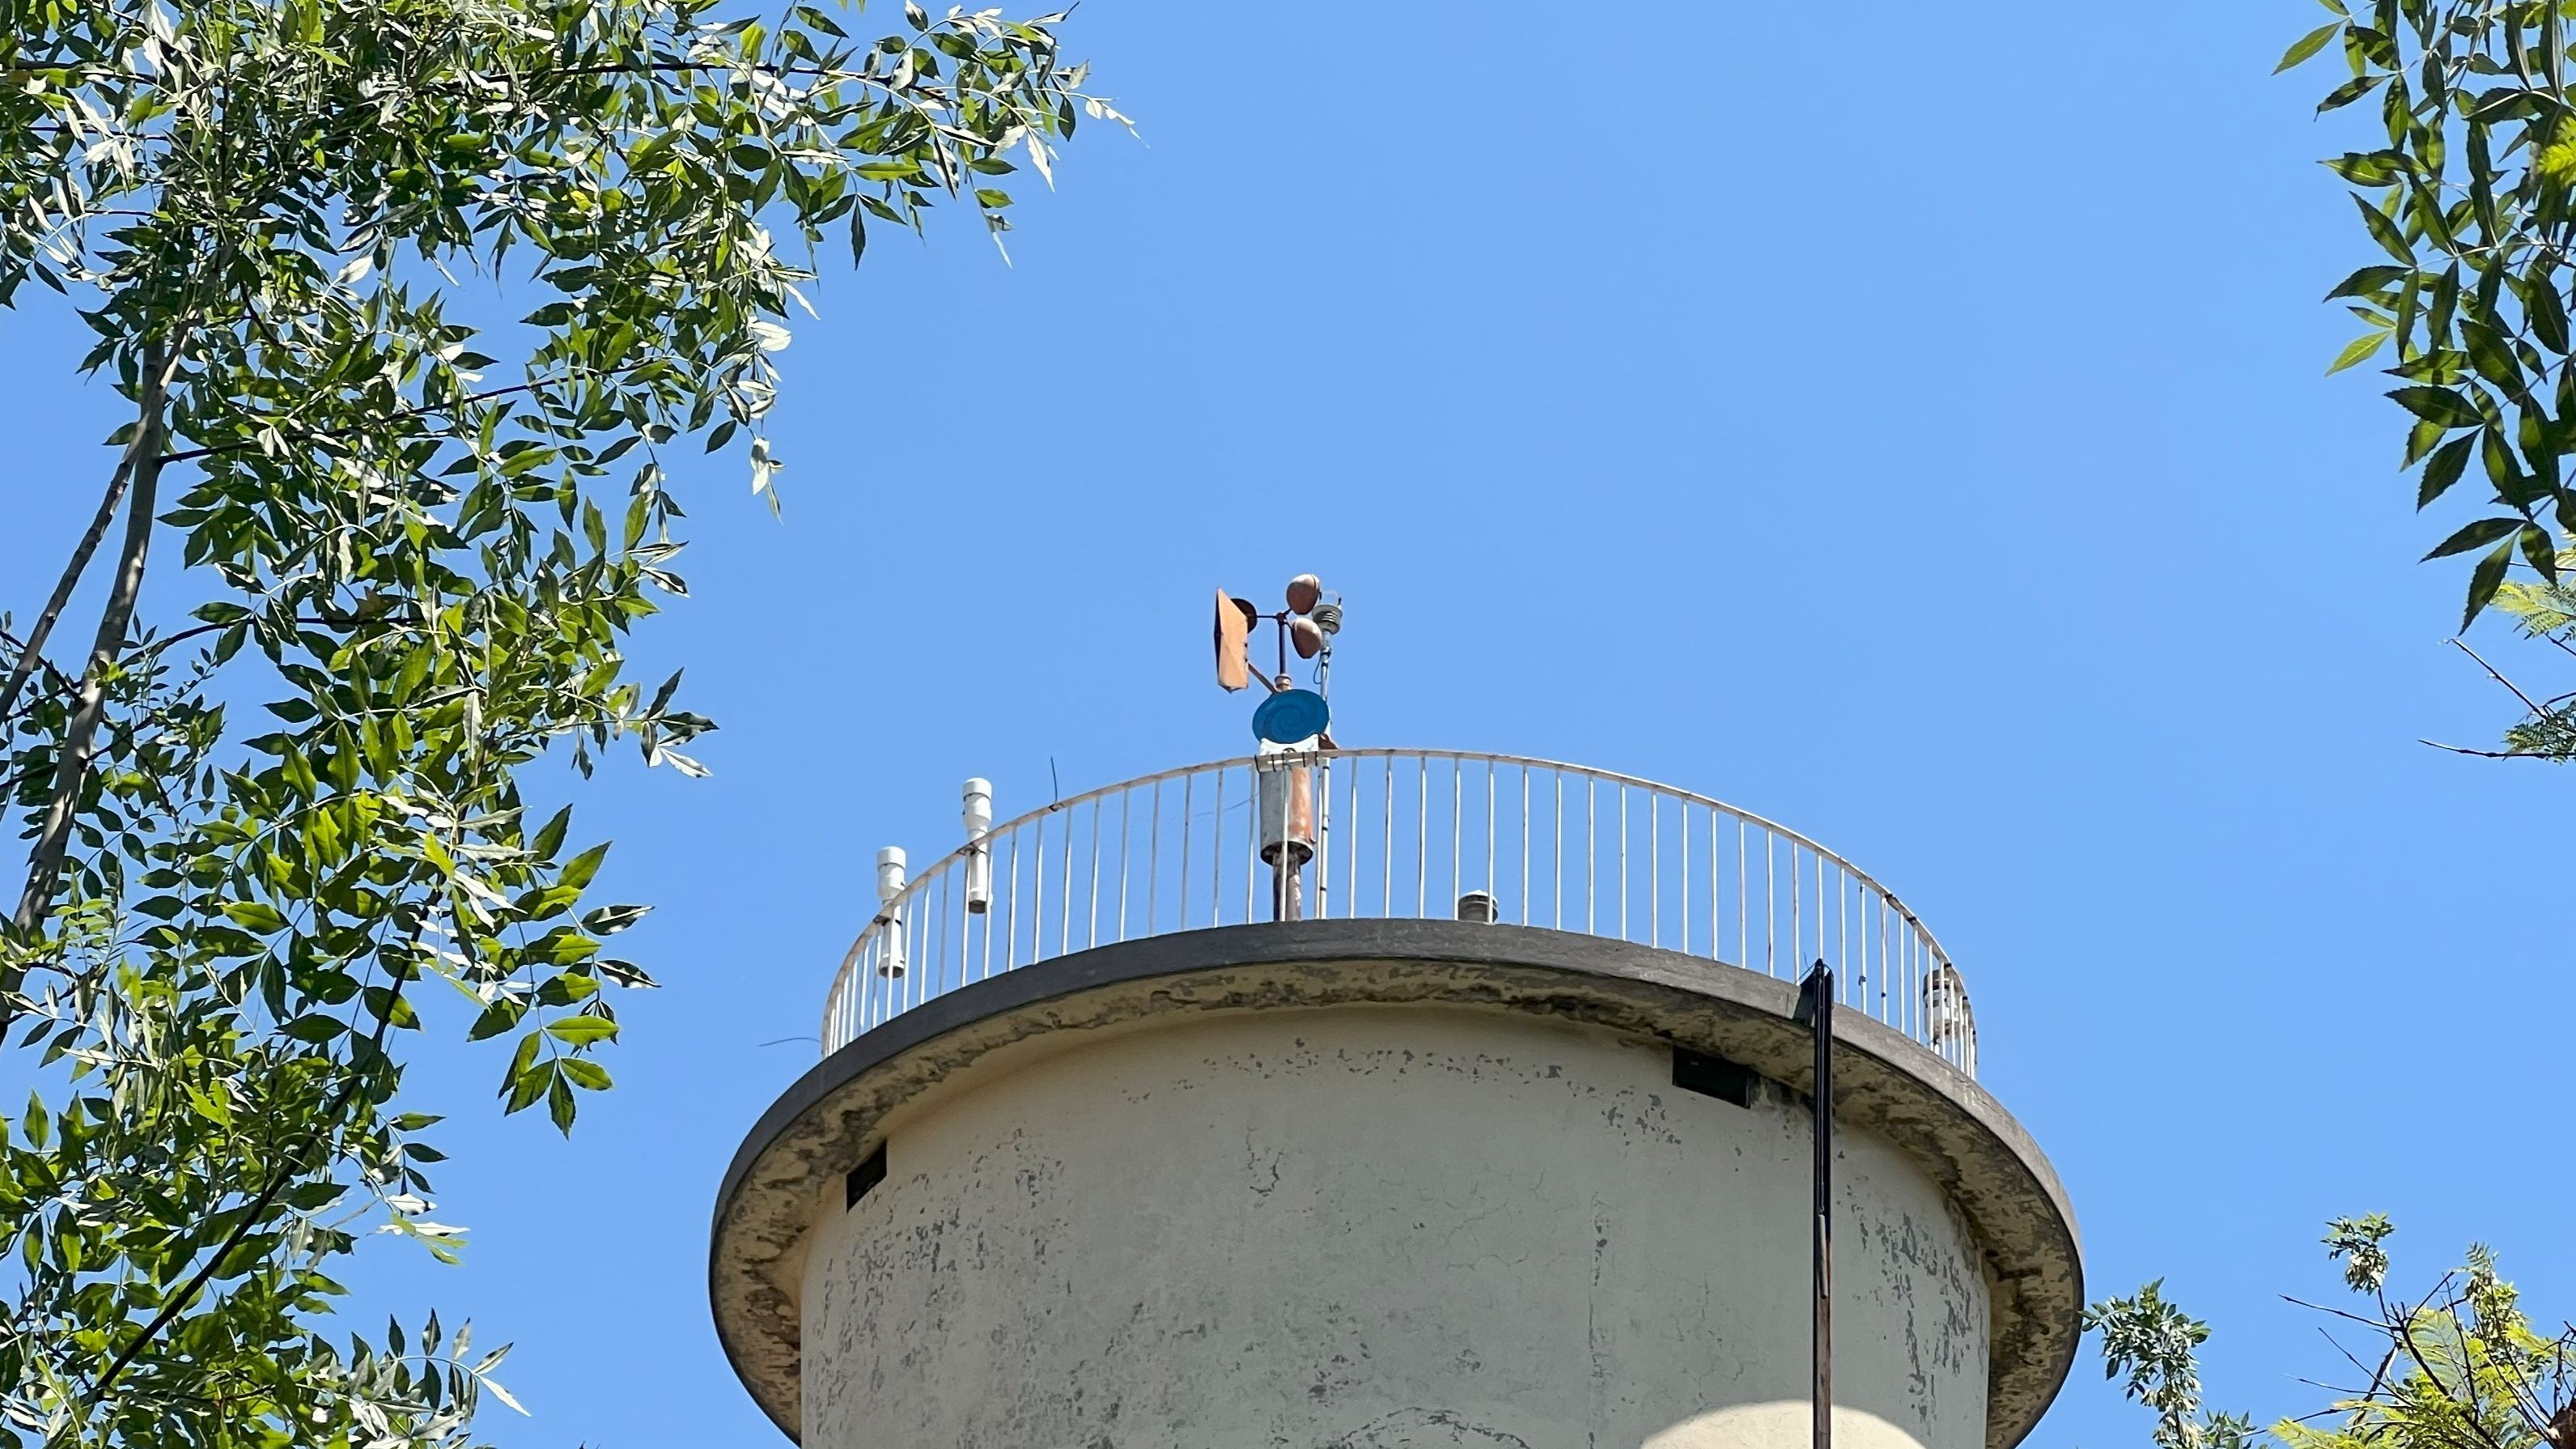
\includegraphics[width=\textwidth]{img/fake_star}
        \caption{Antena de la estrella artificial instalada en la copa de agua.}
        \label{fig:antena_estrella2}
    \end{subfigure}
\end{figure}

La antena de la estrella artificial se encuentra a una altura de 15 metros sobre el suelo y a 186 metros de la antena del telescopio. La antena de la estrella artificial es una antena de polarización circular de alto ancho de banda con una ganancia de 3 dBi aproximadamente.\\

La línea de vista de la antena se encuentra totalmente despejada, manteniendo la primera zona de Fresnel libre de obstáculos para las frecuencias de interés.\\

Como generador de señales se utilizó un generador Valon 5008 con una salida de 2.23 dBm a 1428 MHz y a 400 MHz. Además, se le instaló un filtro pasabajo para minimizar la presencia de los armónicos de alta frecuencia evitando la generación innecesaria de RFI.\\

\begin{figure}
    \centering
    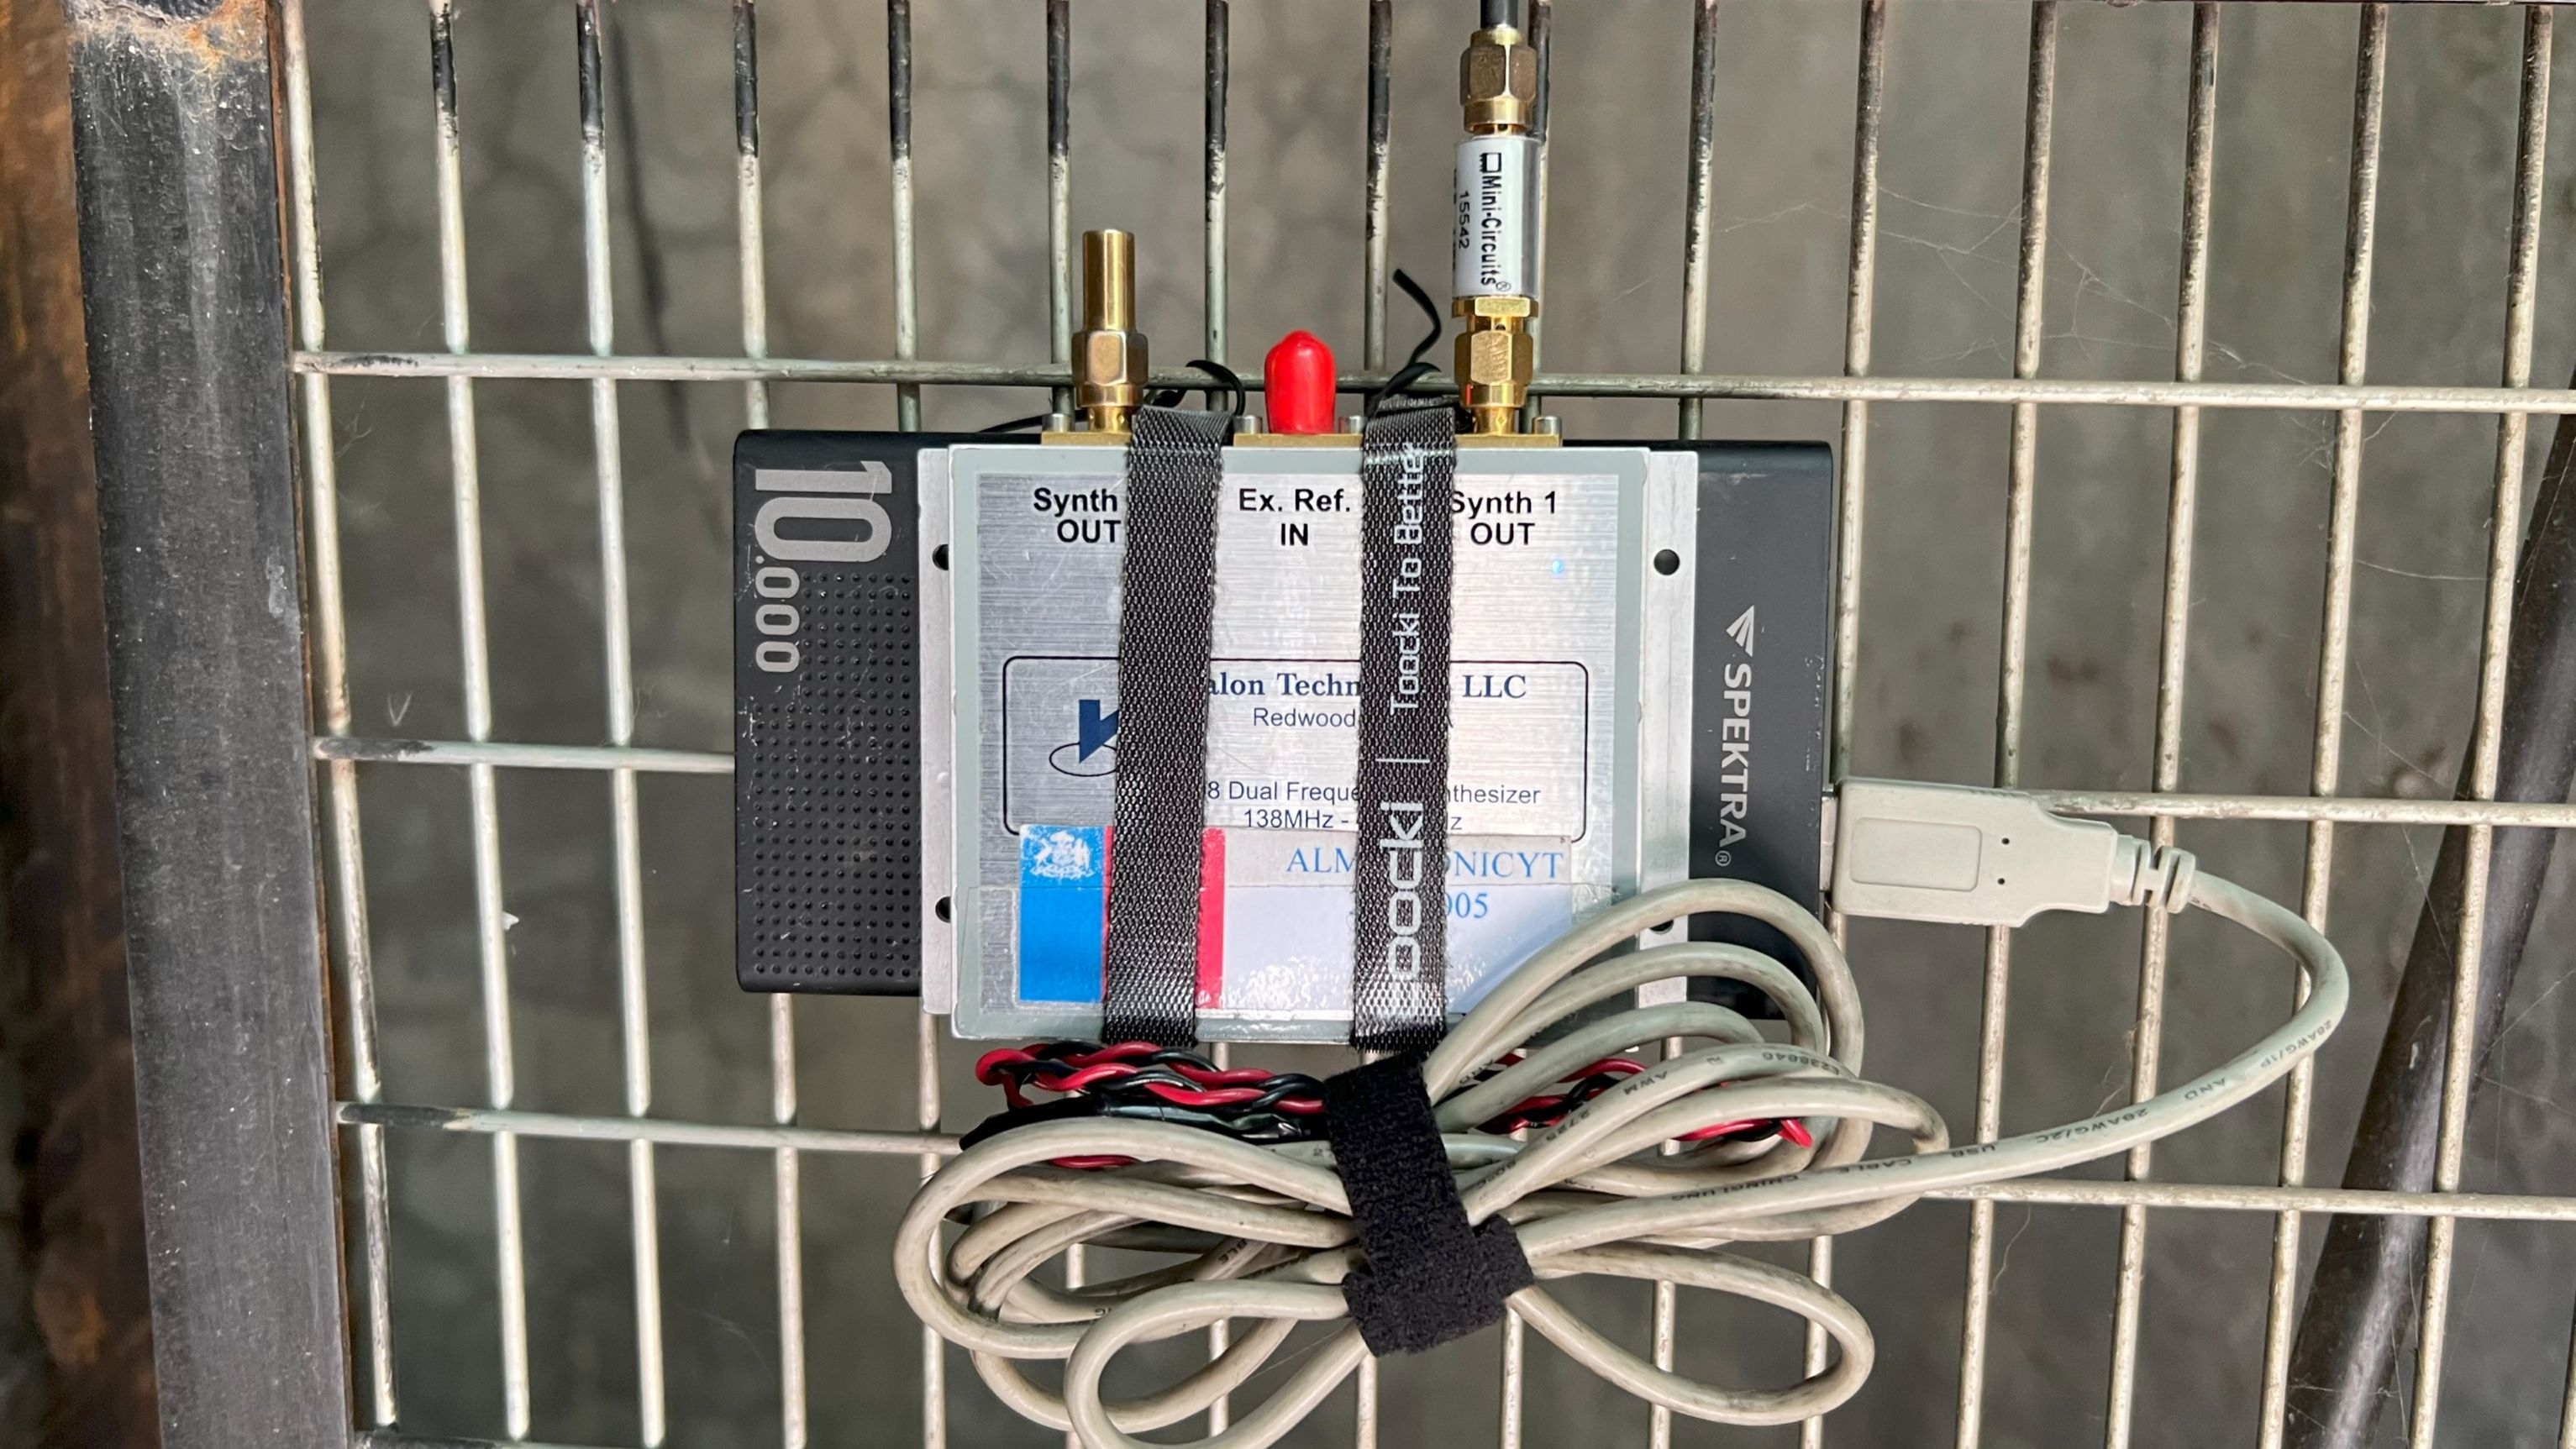
\includegraphics[width=0.8\textwidth]{img/valon}
    \caption{Generador de señales Valon 5008 con filtro pasabajo con una batería externa.}
    \label{fig:generador}
\end{figure}

El generador de la figura \ref{fig:generador} se conecta a la antena de la estrella artificial por medio de un cable coaxial de 20 metros de longitud y se alimenta por una batería externa de 5 V. Se programa previamente la frecuencia a la que se requiera para las mediciones.\\

\subsection{Fuente de ruido}

Para realizar la medición de la temperatura de ruido se requirió de una fuente de ruido. Para obtener la temperatura de la cadena de recepción se utilizó una fuente de ruido Agilent 346B con una alimentación de 28 V.\\

\begin{figure}
    \centering
    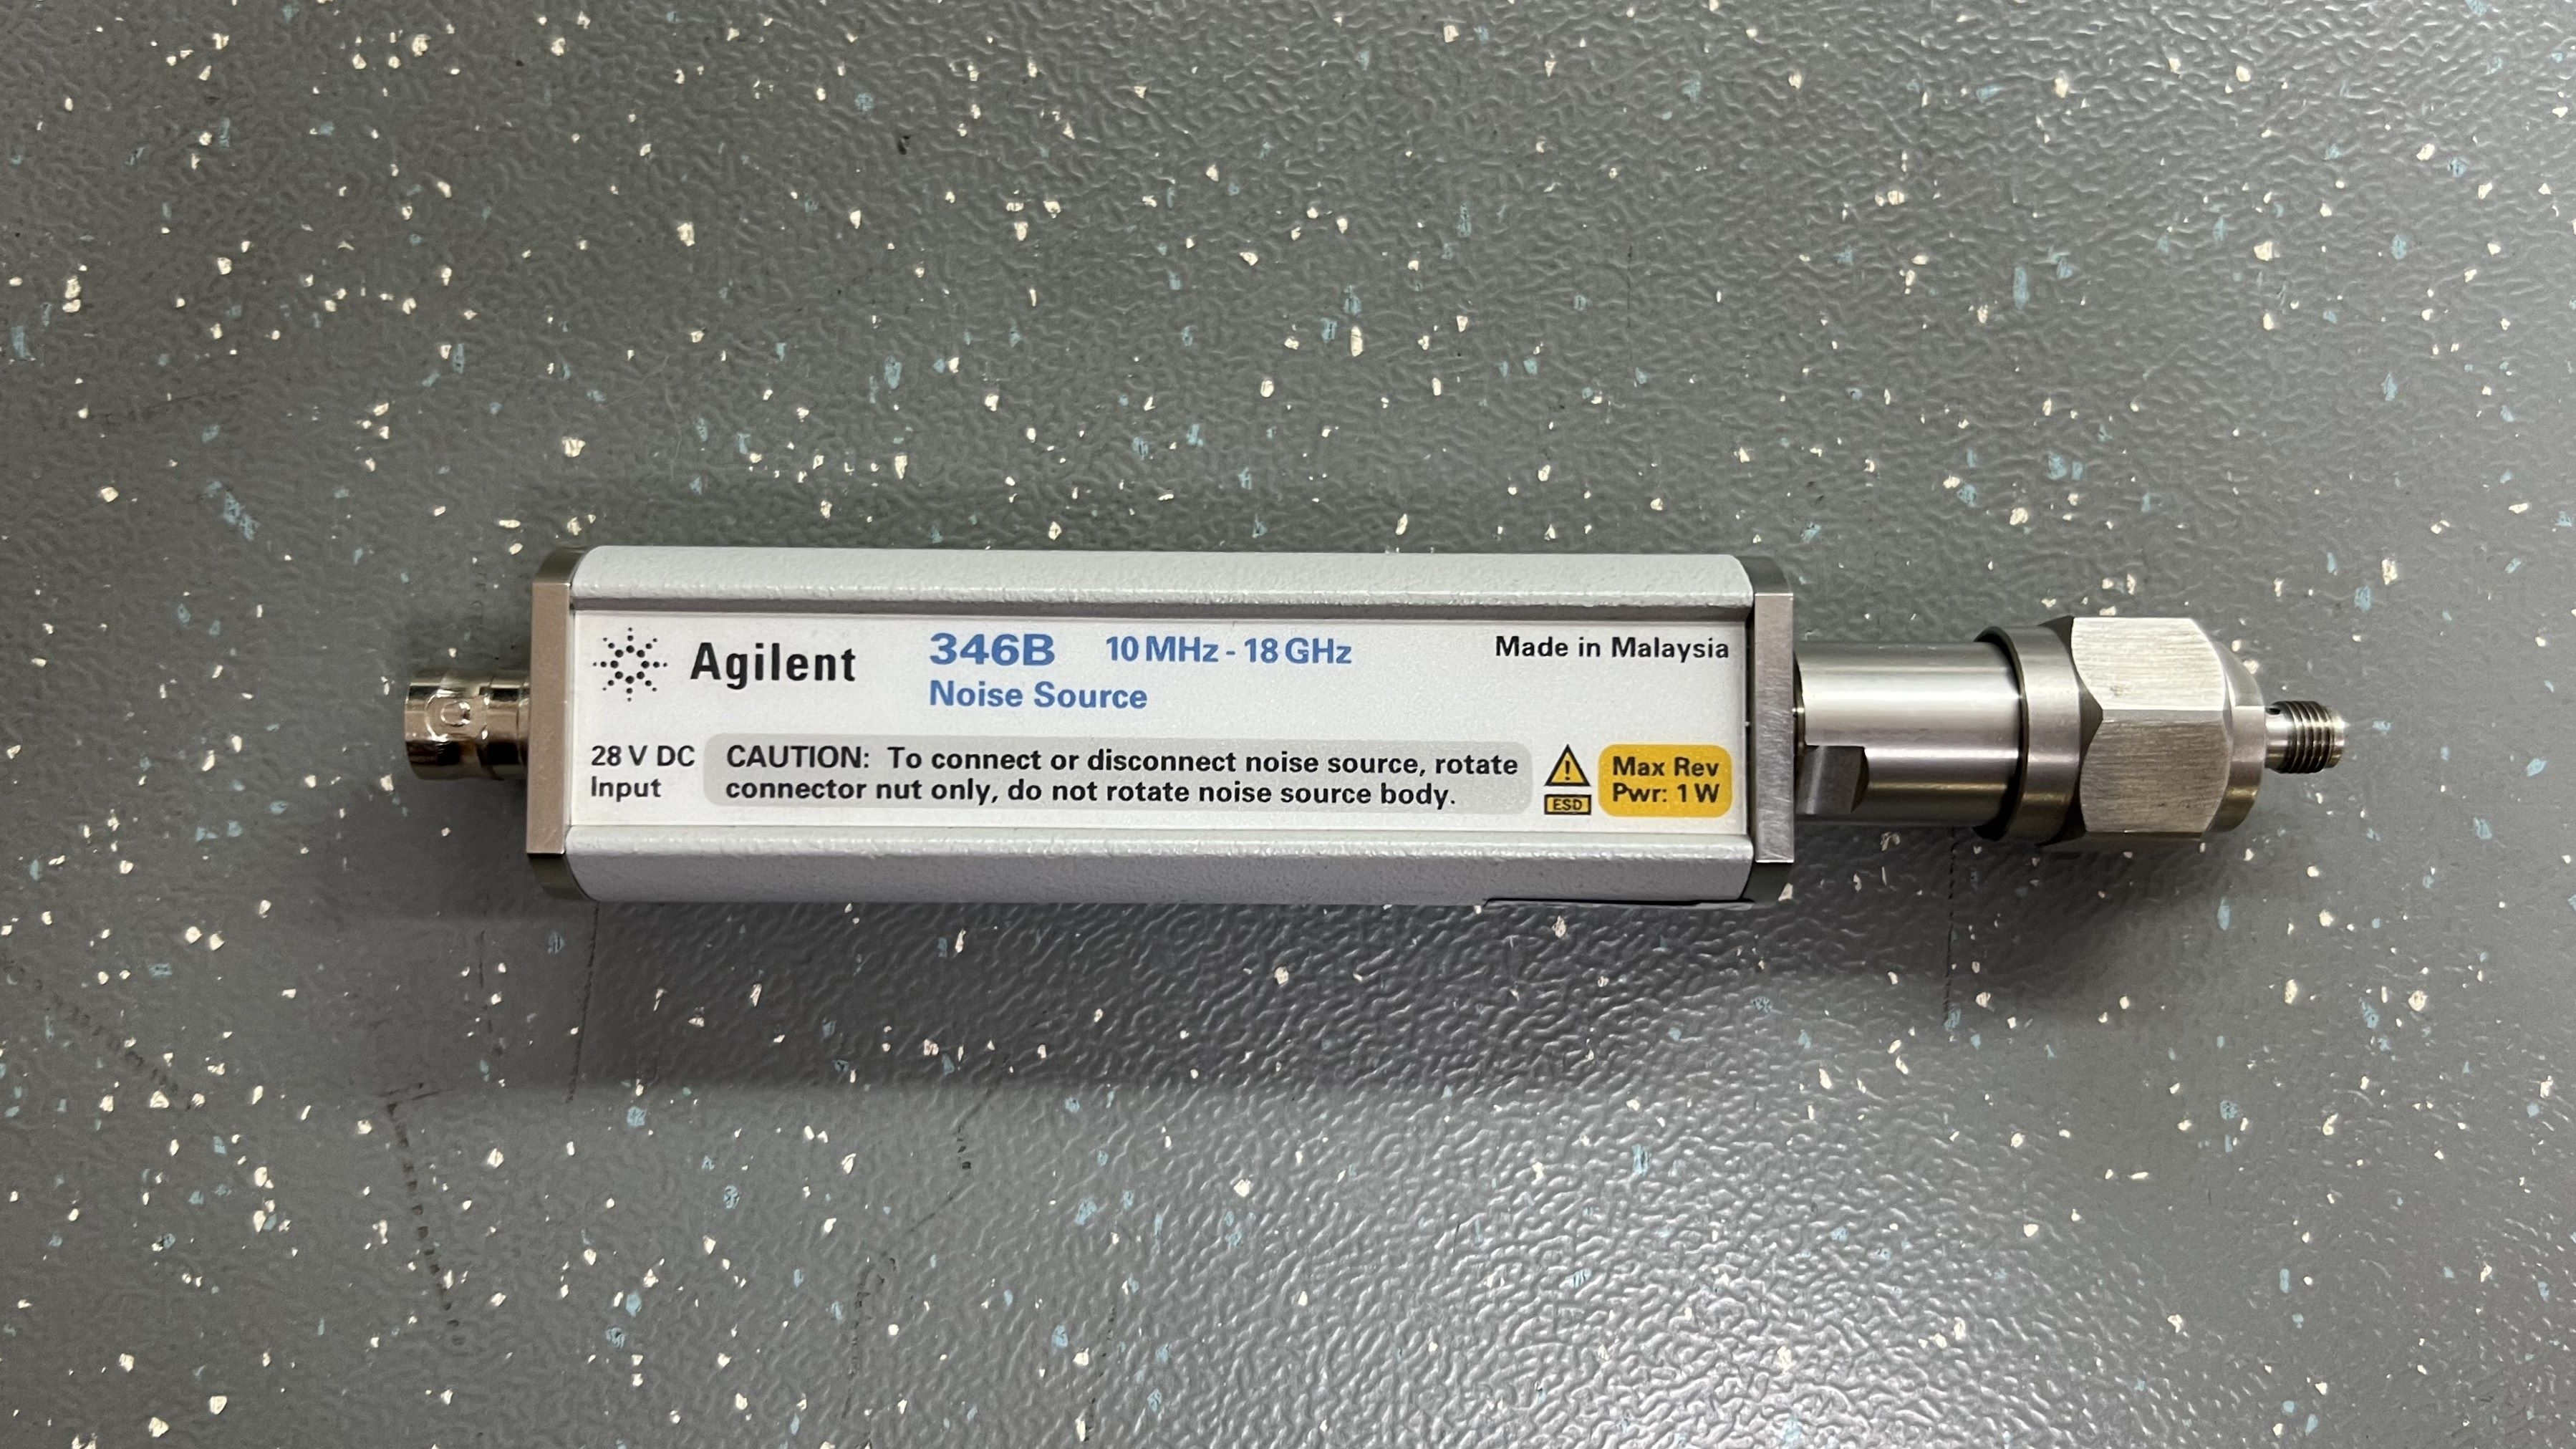
\includegraphics[width=0.8\textwidth]{img/fuenteRuido}
    \caption{Fuente de ruido Agilent 346B.}
    \label{fig:fuente_ruido}
\end{figure}

\subsection{Software de caracterización}

\paragraph{cpt\_rp\_measure.py} Es un software que al igual que los de la sección \ref{sec:software} obtiene espectros y los guarda para el análisis futuro. La diferencia es que este software está diseñado para la calibración del instrumento, por lo que además este instrumento guarda los espectros tomados por ángulo con respecto a la estrella artificial de la copa de agua para las mediciones de patrón de radiación.\\

Este script genera un archivo con los espectros tomados por ángulo y luego mueve la montura a otro ángulo para tomar otro espectro, este proceso se repite hasta que se obtienen un corte de 180 grados con la cantidad de espectros que haya sido configurada.\\

Como la fuente de calibración se encuentra en altura, hay que ajustar el plano de rotación con respecto a plano azimutal de la montura, para esto se utilizó la siguiente conversión de coordenadas:\\

\begin{equation}
    \theta' = \theta + \left(1- \frac{2\phi}{\pi}\right)E
\end{equation}

\begin{equation}
    \phi' = \phi
\end{equation}

Donde $\theta$ es la elevación original, $E$ es el ángulo de elevación de la estrella artificial con respecto a la antena, $\phi$ es el azimut, $\theta'$ y $\phi'$ son las nuevas coordenadas. Con esta conversión se tiene una elevación específica para cada punto de azimut que permite mantener el plano de rotación de la fuente de calibración en el nuevo plano de azimutal.\\

\paragraph{cpt\_siglent.py} Es un software que utiliza de manera remota el instrumento Siglent SVA1075X para obtener sus espectros y realizar las mismas mediciones de patrón de radiación que el software anterior.\\